\label{sec:gbb-bkgsub}
\subsection{Flavor Fractions}
Post \btagging, a large fraction of events are backgrounds as shown in Table~\ref{tab:posttaggingflav}. To unfold the data, subtraction of the remnant background is necessary. It is a known problem that the nominal MC flavor fractions could deviate from the true values in data (see e.g.~\cite{ATLAS-CONF-2016-002}). To have good control over the flavor fractions, we seek to estimate the flavor fractions in bins of each observable by fitting the distributions of some variables, which may not be powerful enough to tag individual jets, but are sensitive to the numbers of jets of different flavors. 

\begin{table}[htbp]
\centering
\resizebox{\textwidth}{!}{
\begin{tabular}{|l|l|l|l|l|l|l|l|l|l|}
\hline
Flavor Combination & BB      & BC     & BL     & CB     & CC     & CL     & LB     & LC     & LL     \\ \hline
Flavor Fraction    & 19.01\% & 2.20\% & 34.68\% & 0.39\% & 5.73\% & 17.99\% & 0.37\% & 0.86\% & 18.76\% \\ \hline
\end{tabular}}
\caption{Post $b$-tagging flavor composition in MC. The first letter of the flavor combination is the flavor of the leading jet. The second letter of the combination is the flavor of the sub-leading jet. }
\label{tab:posttaggingflav}
\end{table}


\subsection{$s_{d_{0}}$ as Discriminant Variable }
\label{sec:gbb-sd0}

The long decay length of heavy flavor hadrons make the signed significance of impact parameter $s_{d_{0}}$ of tracks associated to a jet a good discriminating variable. The $s_{d_{0}}$ is defined as 
\begin{equation}
s_{d_{0}} = \frac{d_0}{\sigma(d_0)} \cdot s_{j}
\end{equation}
where $d_{0}$ is the track transverse impact parameter, $\sigma(d_{0})$ is the uncertainty on the $d_0$ measurement, and $s_{j}$ is the sign of $d_{0}$ with respect to the jet axis. The variable $s_j$ is defined as
\begin{equation}
s_{j} = \textrm{sign}\left\{\ \sin\left(\arctan \left( \frac{p_{j,\ y}}{p_{j,\ x}}\right) - \phi_t\right) \cdot d_{0} \ \right\}
\end{equation}
 where $p_{j,\ x}$ and $p_{j,\ y}$ are the $x$ and $y$ components of the jet moments, respectively, and $\phi_{t}$ is the azimuthal angle of the track.
 
For a given track jet, by construction we have at least two tracks as constituents of the jet. %(number of track constituents distributions are shown in Fig.\ref{fig:gbb-ntrk}).
We take the sub-leading $s_{d_{0}}$ of the track (leading means highest value of $|s_{d_{0}}|$, sub-leading is second largest, etc.) as \subsdzero and build templates of different flavors using this variable to fit and derive the flavor fractions from data.   The second highest $s_{d_{0}}$ is used because it is less likely the result of mis-measured track parameters for non-$b$-jets. For illustration of the impact parameter significance please refer back to Fig.\ref{fig:reco-trkdef}.


%\begin{figure}[htbp]
%  \centering
% 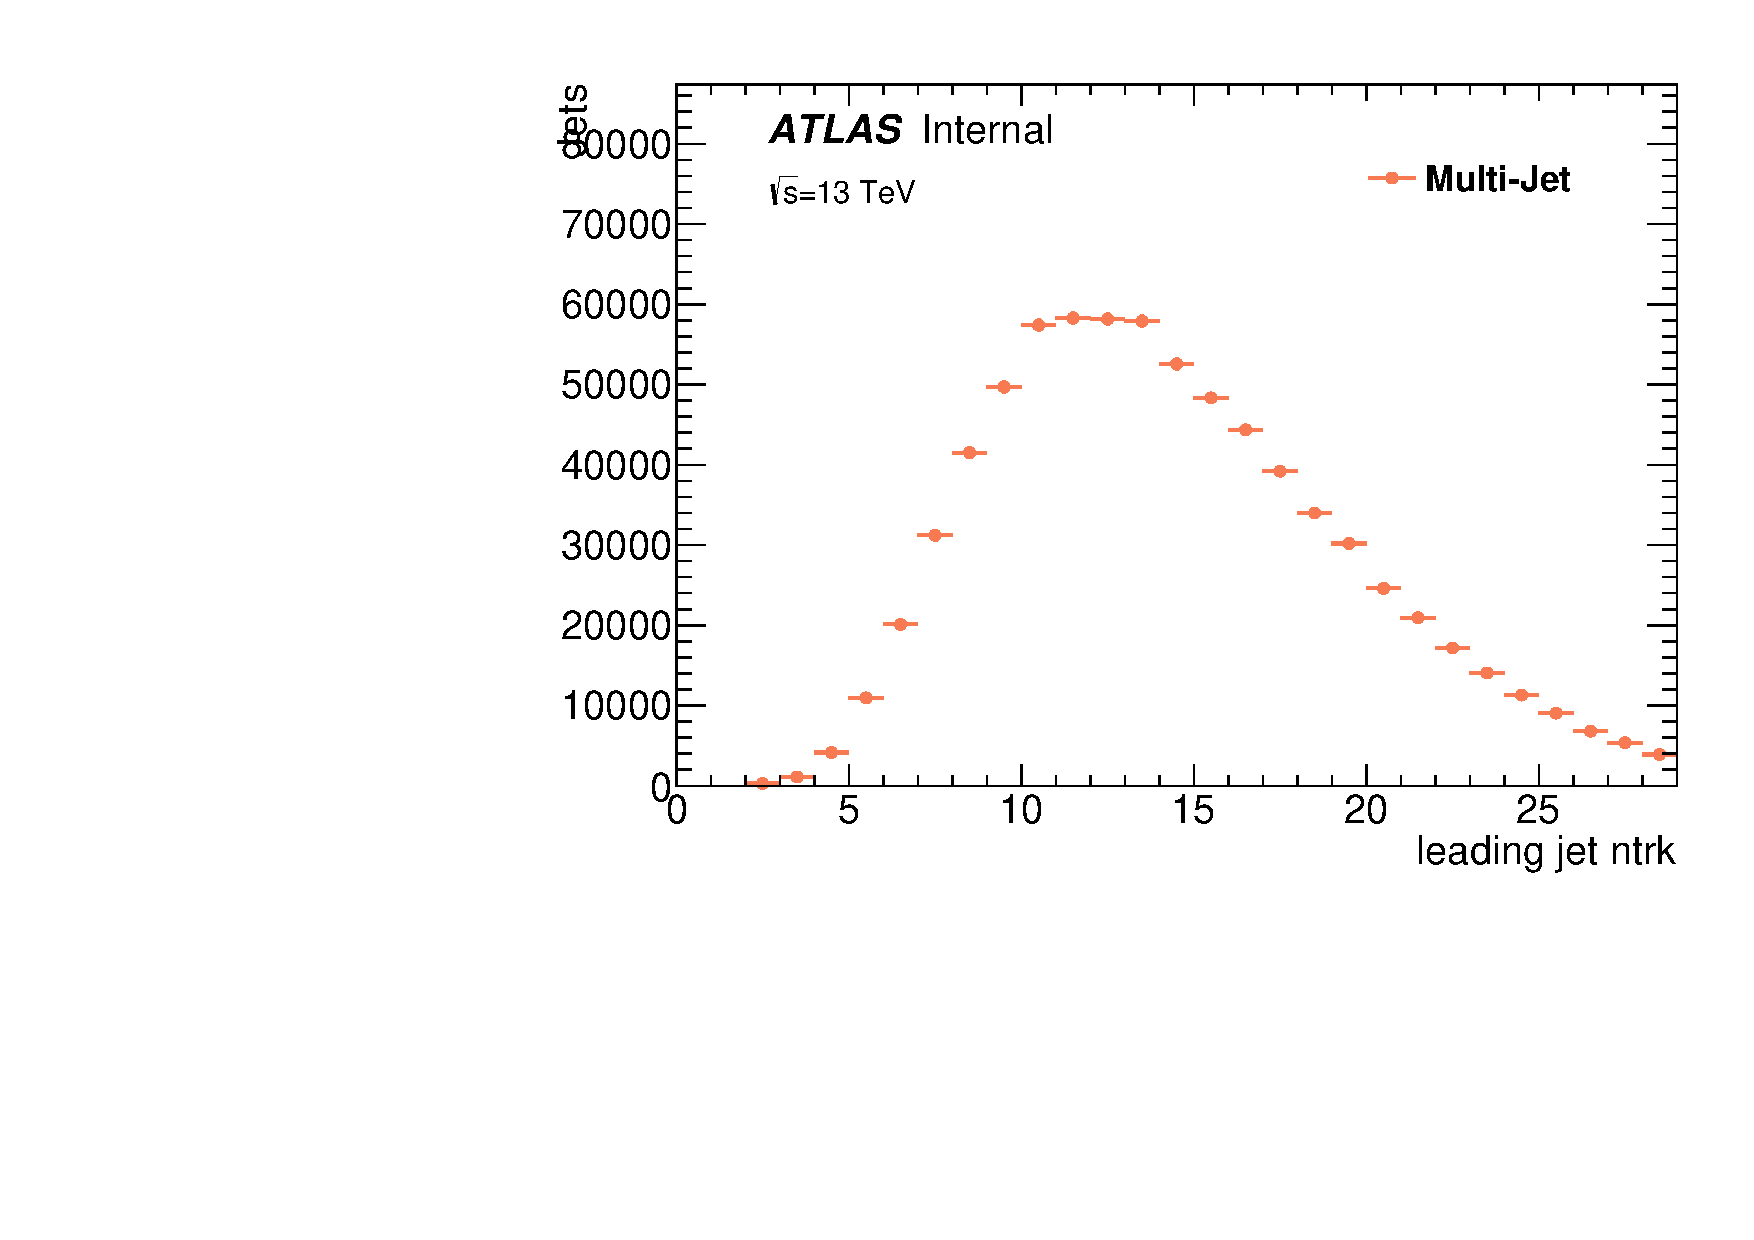
\includegraphics[width=0.48\textwidth]{figures/gbb/Leading_trkjet_ntrk_PostTag.pdf}
% 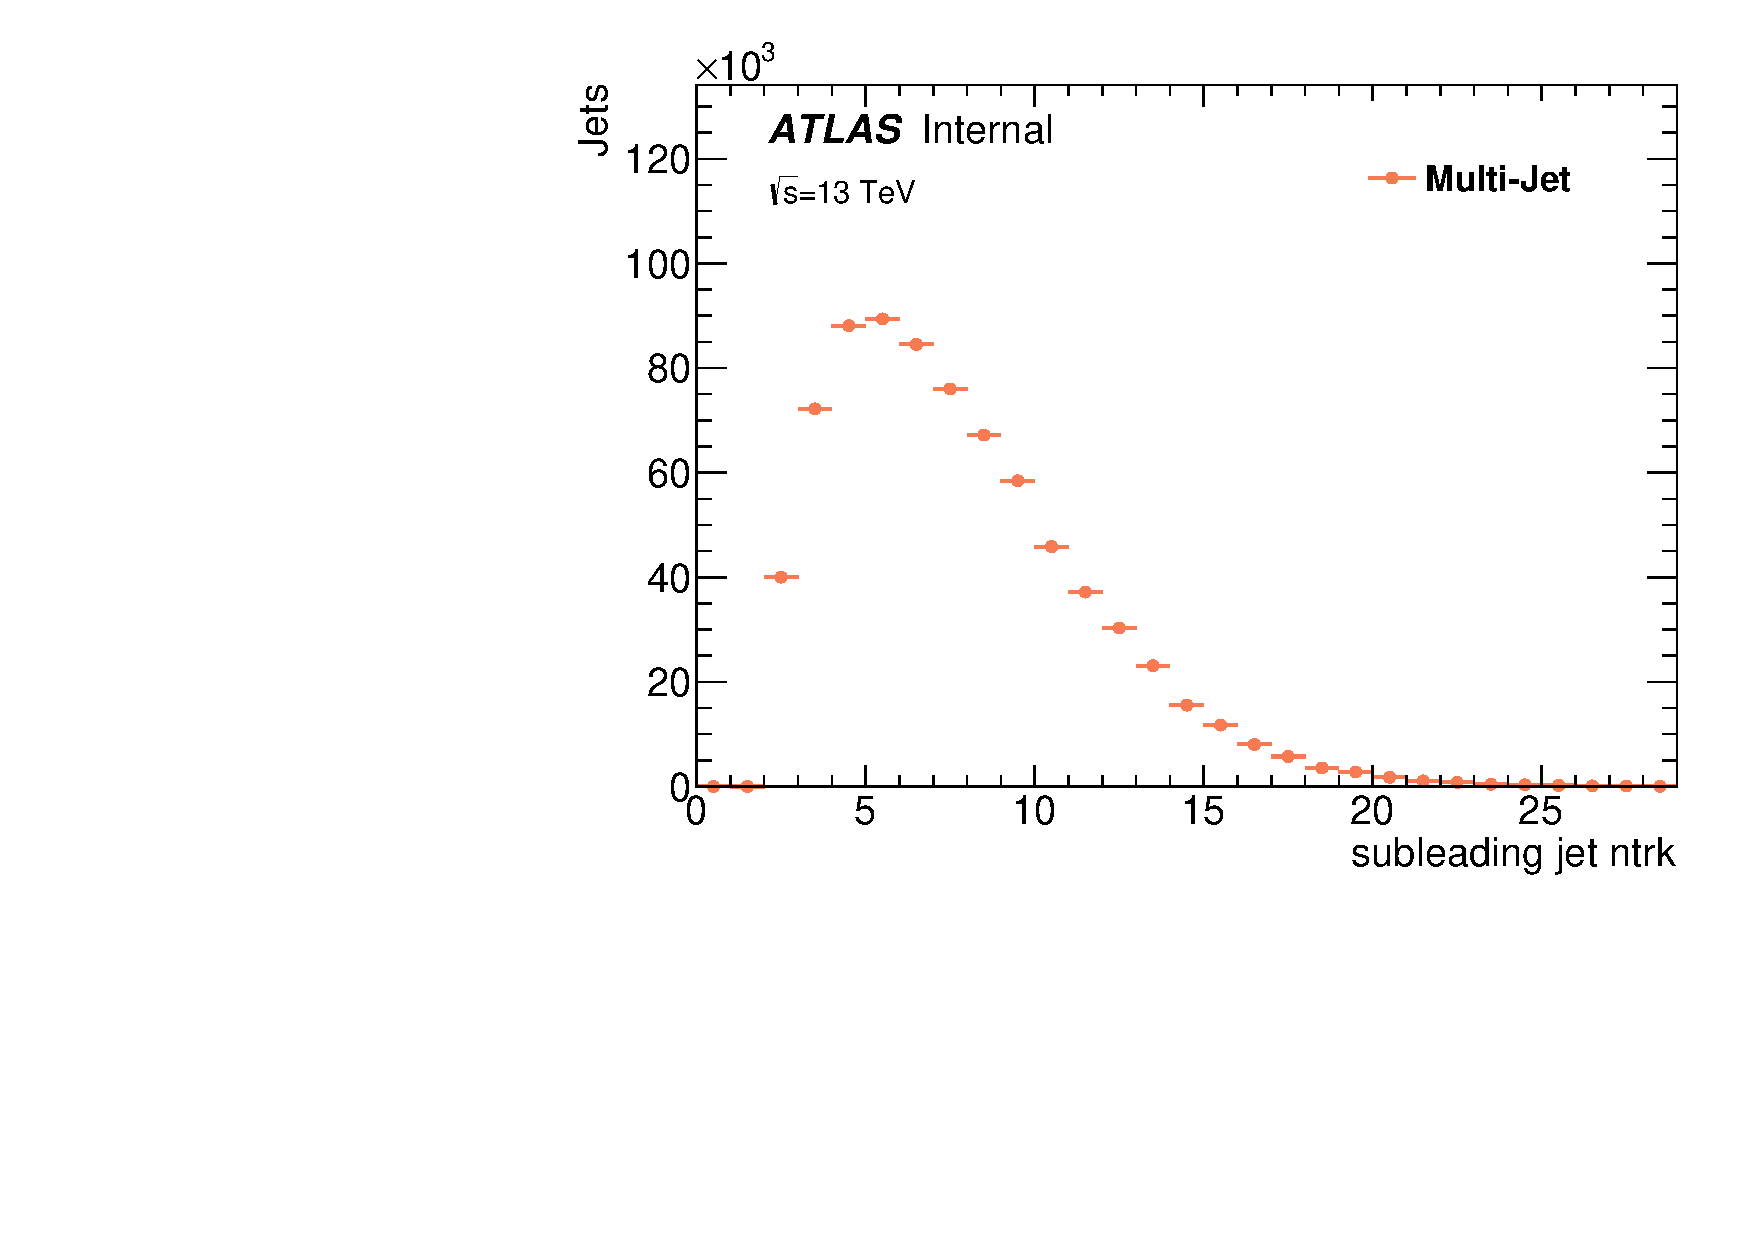
\includegraphics[width=0.48\textwidth]{figures/gbb/SubLeading_trkjet_ntrk_PostTag.pdf}\\
%\caption{The number of track distribution for leading (left) and sub-leading (right) track jets in MC prediction}
%  \label{fig:gbb-ntrk}
%\end{figure}


%%%%%%%%%%%%%%%%%%%%%%%%%%%%%%%%%%%%%%%%%%%%%%%%%

\subsection{Binned Maximum Likelihood Estimation}

An $m$ flavor component template fit ($m = 3$ for the fit we perform) is carried out by maximizing a binned likelihood function defined as $\mathcal{L} = \prod _{i=1} ^n p(y_i| \vec{\theta})$, where $\vec{\theta} \in \mathbb{R}^m$ denotes the number of events from each flavor component, $n$ is the number of bins we are fitting and $y_i$ is the number of data events in bin $i$. The assumption of $p(y_i|\vec{\theta})$ is Poisson distribution: 
\begin{equation}
p(y_i|\vec{\theta}) = \frac{\exp{(-\vec{\theta} \vec{\cdot x_i)}} {(\vec{\theta}} \vec{\cdot x_i})^{y_i}}{y_i !}, 
\end{equation}
where $\vec{x_i}=(x_{i1}...,x_{ij}...,x_{im}) \in \mathbb{R}^m$ is a vector, and each component denotes the $i^{th}$ bin value in the normalized templates for the $j^{th}$ flavor ($b$, $c$ and light).   We determine the flavor fractions by finding the $\vec{\theta}$ that maximizes $\mathcal{L}$. The fit is carried out by the MIGRAD function of the MINUIT package. 

%%%%%%%%%%%%%%%%%%%%%%%%%%%%%%%
\subsection{\subsdzero Templates }
\label{sec:gbb-subdzerotemplates}

The flavor contents of the two $R=0.2$ jets in a $R=1.0$ jet are correlated. 
Tagging one of the $b$ jets increases the probability of the other track jet 
being a $b$ jet. Therefore, we should not treat the flavor 
contents of the two jets independently and thus must take into account both jets 
flavors simultaneously when fitting. On the other hand, given the flavors of the 
two $R= 0.2$ jets, their \subsdzero values are not correlated, as shown in Table \ref{tab:sd0cor}. 
Therefore, we can derive the flavor fractions by fitting simultaneously the 
1-dimensional \subsdzero distributions of the leading and sub-leading jets
 using templates derived from all of the possible 2-jet flavor pair 
combinations. This is essentially a Naive Bayes approximation, i.e. assuming the joint 
2-D probability density is the product of the two 1-D probability density
 $p(\subsdzero(j1), \subsdzero(j2)) = p(\subsdzero(j1))p(\subsdzero(j2))$.

\begin{table}[htbp]
\centering
\begin{tabular}{|r|r|r|r|}
\hline
\centering
Flavor Combination & \subsdzero Correlation Factor\\
\hline
BB & 0.7\% \\
BL & 0.4\% \\
BC & -2.2\% \\
LB & 3.9\%\\
LL & 0.3\%\\
LC & 0.8\%\\
CB & -0.3\% \\
CL & 0.5\% \\
CC & -4.1\% \\

\hline
\end{tabular}%
\caption{Correlation factor between the \subsdzero values of the two R = 0.2 jets.}
\label{tab:sd0cor}
\end{table}%

There are in total nine different ordered flavor pairs: BB, BL, BC, CB, CL, CC, 
LB, LC and LL such that the first flavor is that of the leading track jet and 
the second is that of the other track jet. Many of these components are very small 
for us to fit their contributions correctly as show in Table~\ref{tab:posttaggingflav}. 
Therefore, starting with BL, CL templates, we merge other templates to these templates
to form B-like and C/L-like templates. The metric we use for determining the similarity 
between two distributions is: $S=\frac{1}{2}\int \frac{(p_1(x)-p_2(x))^2}{p_1(x)+p_2(x)}$, 
where $p_1(x)$ and $p_2(x)$ are two different distributions. 
Based on calculation, we merge the BC template with the BL 
template, and other components into CL as seen in 
Table \ref{tab:overlap-unmerged}. The merged templates are 
presented in Figure \ref{fig:gbb-templates} and the separation powers estimated by the same metric are 
presented in Table \ref{tab:overlap-merged}. 
We show the full set of templates in bins of the observables we are interested in 
measuring in Appendix~\ref{sec:gbb-app-sd0templates}. 

It is noteworthy that the statistics of our Monte Carlo samples is low.
Presumably, a double $b$-tagging strategy would be preferable as it could filter 
out most of the background processes.
However, double $b$-tagging strategy would also yield background templates with large 
statistical fluctuations. In Fig. \ref{fig:gbb-template-leadtight-medium} the comparison 
of the templates derived from single $b$-tagging and double $b$-tagging (at 70\% $b$-
efficiency for both jets) in one bin of $\Delta R$ is shown. The considerable statistical uncertainties ($\geq 10\%$ relative uncertainty per bin in template)
of double $b$-tagging strategy lead us to use single $b$-tagging strategy instead. 


\begin{table}[htpb]
\centering
\begin{tabular}{|l|l|l|l|l|}
\hline
   & BL   & CL    & BB   \\ \hline
BC & 0.02 & 0.08  & 0.11 \\ \hline
CC & 0.09 & 0.03  & 0.14 \\ \hline
LC & 0.07 & 0.05  & 0.12 \\ \hline
LB & 0.17 & 0.12  & 0.05 \\ \hline
CB & 0.19 & 0.14  & 0.08 \\ \hline
LL & 0.02 & 0.01  & 0.17 \\ \hline
BB & 0.16 & 0.21  & 0    \\ \hline

\end{tabular}
\caption{Templates similarity calculated using the metric $S=\frac{1}{2}\int \frac{(p_1(x)-p_2(x))^2}{p_1(x)+p_2(x)}$ for un-merged templates. Given two distributions $p_1(x)$ and $p_2(x)$, the metric returns 0 if they are exactly the same and returns 1 if there is no overlap between them.}
\label{tab:overlap-unmerged}
\end{table}



\begin{table}[htpb]
\centering
\begin{tabular}{|l|l|l|l|l|}
\hline
    & B    & L+C    & BB   \\ \hline
B   & 0    & 0.04  & 0.16 \\ \hline
L+C & 0.04 & 0     & 0.17 \\ \hline
BB  & 0.16 & 0.17  & 0    \\ \hline

\end{tabular}
\caption{Templates similarity calculated using the metric $S=\frac{1}{2}\int \frac{(p_1(x)-p_2(x))^2}{p_1(x)+p_2(x)}$ for merged templates. Given two distributions $p_1(x)$ and $p_2(x)$, the metric returns 0 if they are exactly the same and returns 1 if there is no overlap between them.}
\label{tab:overlap-merged}
\end{table}


\begin{figure}[htbp]
  \centering
 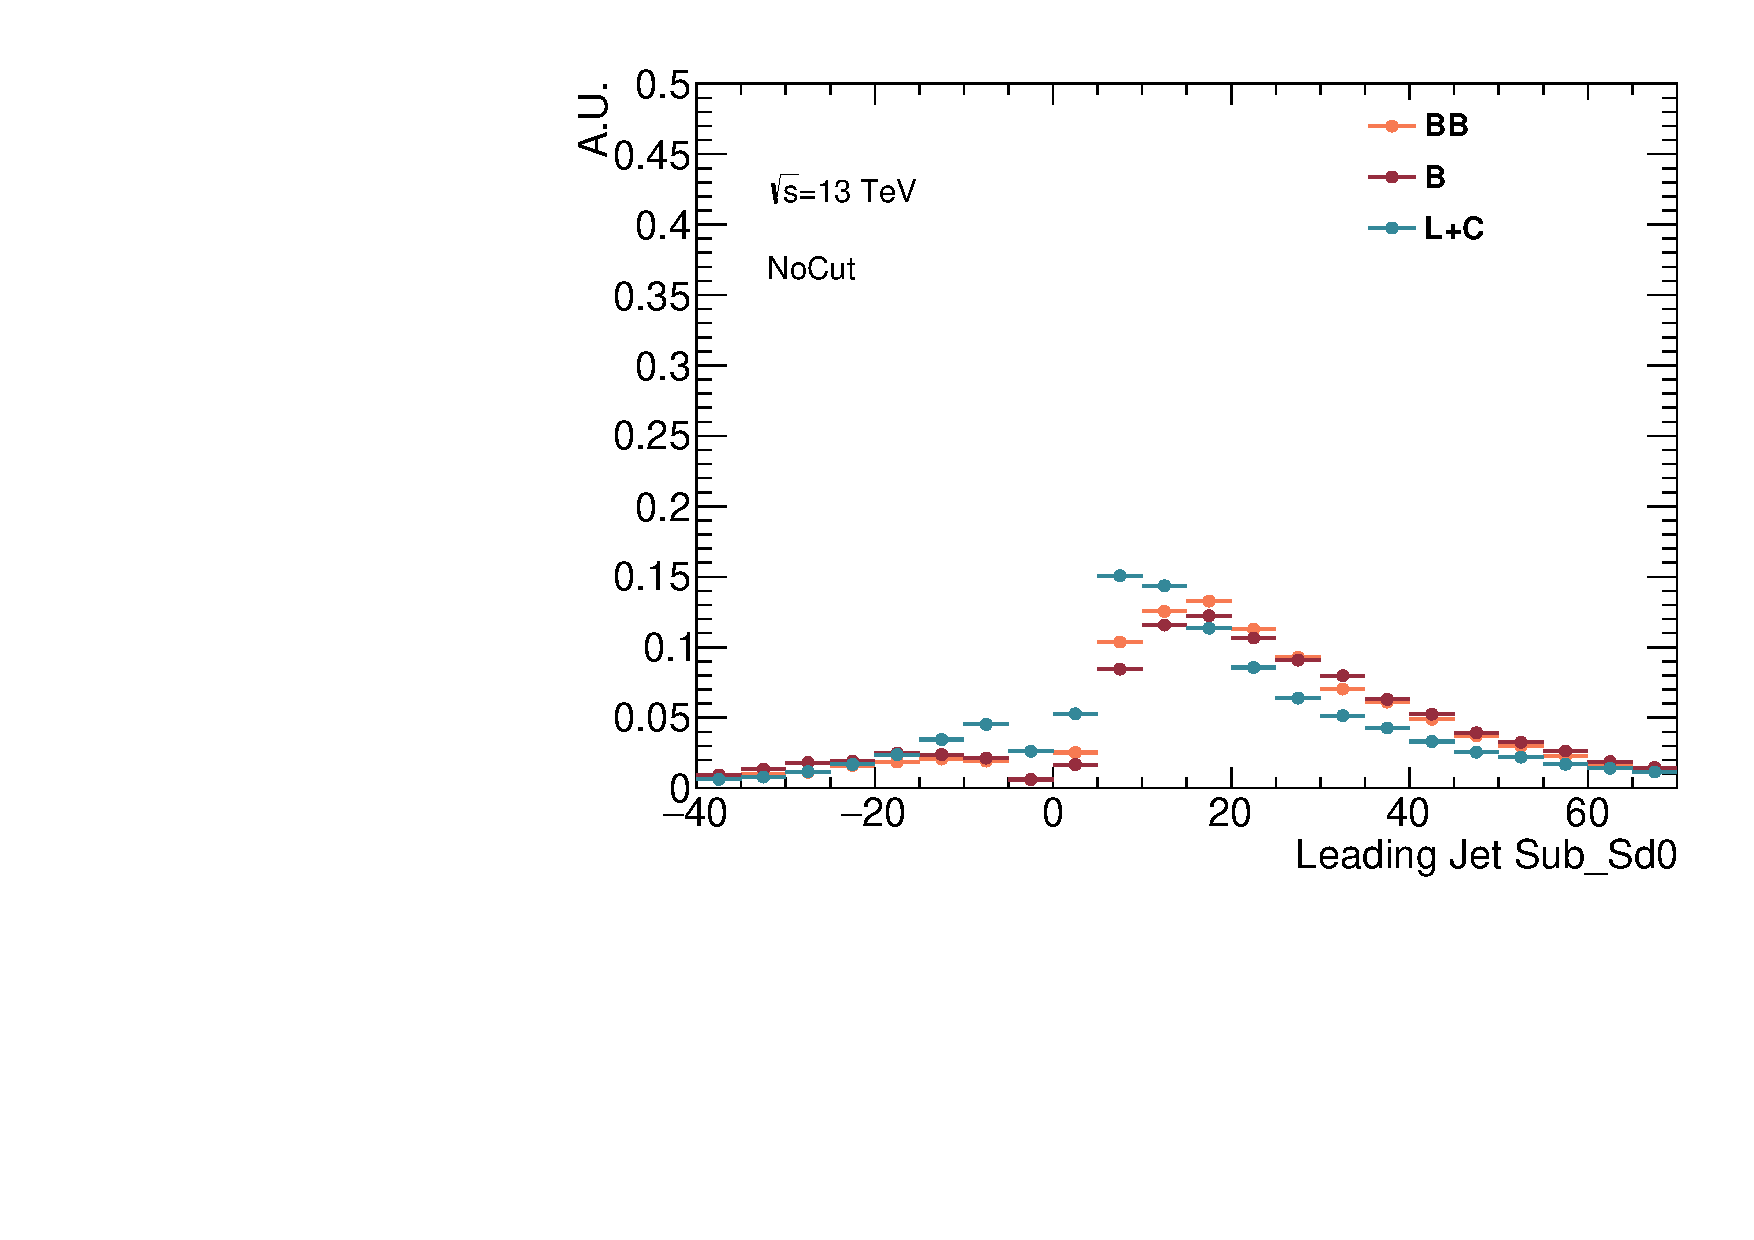
\includegraphics[width=0.48\textwidth]{figures/gbb/Sub_Sd0_Fits/Canv_FitTemplate_Inclusive_x.pdf}
 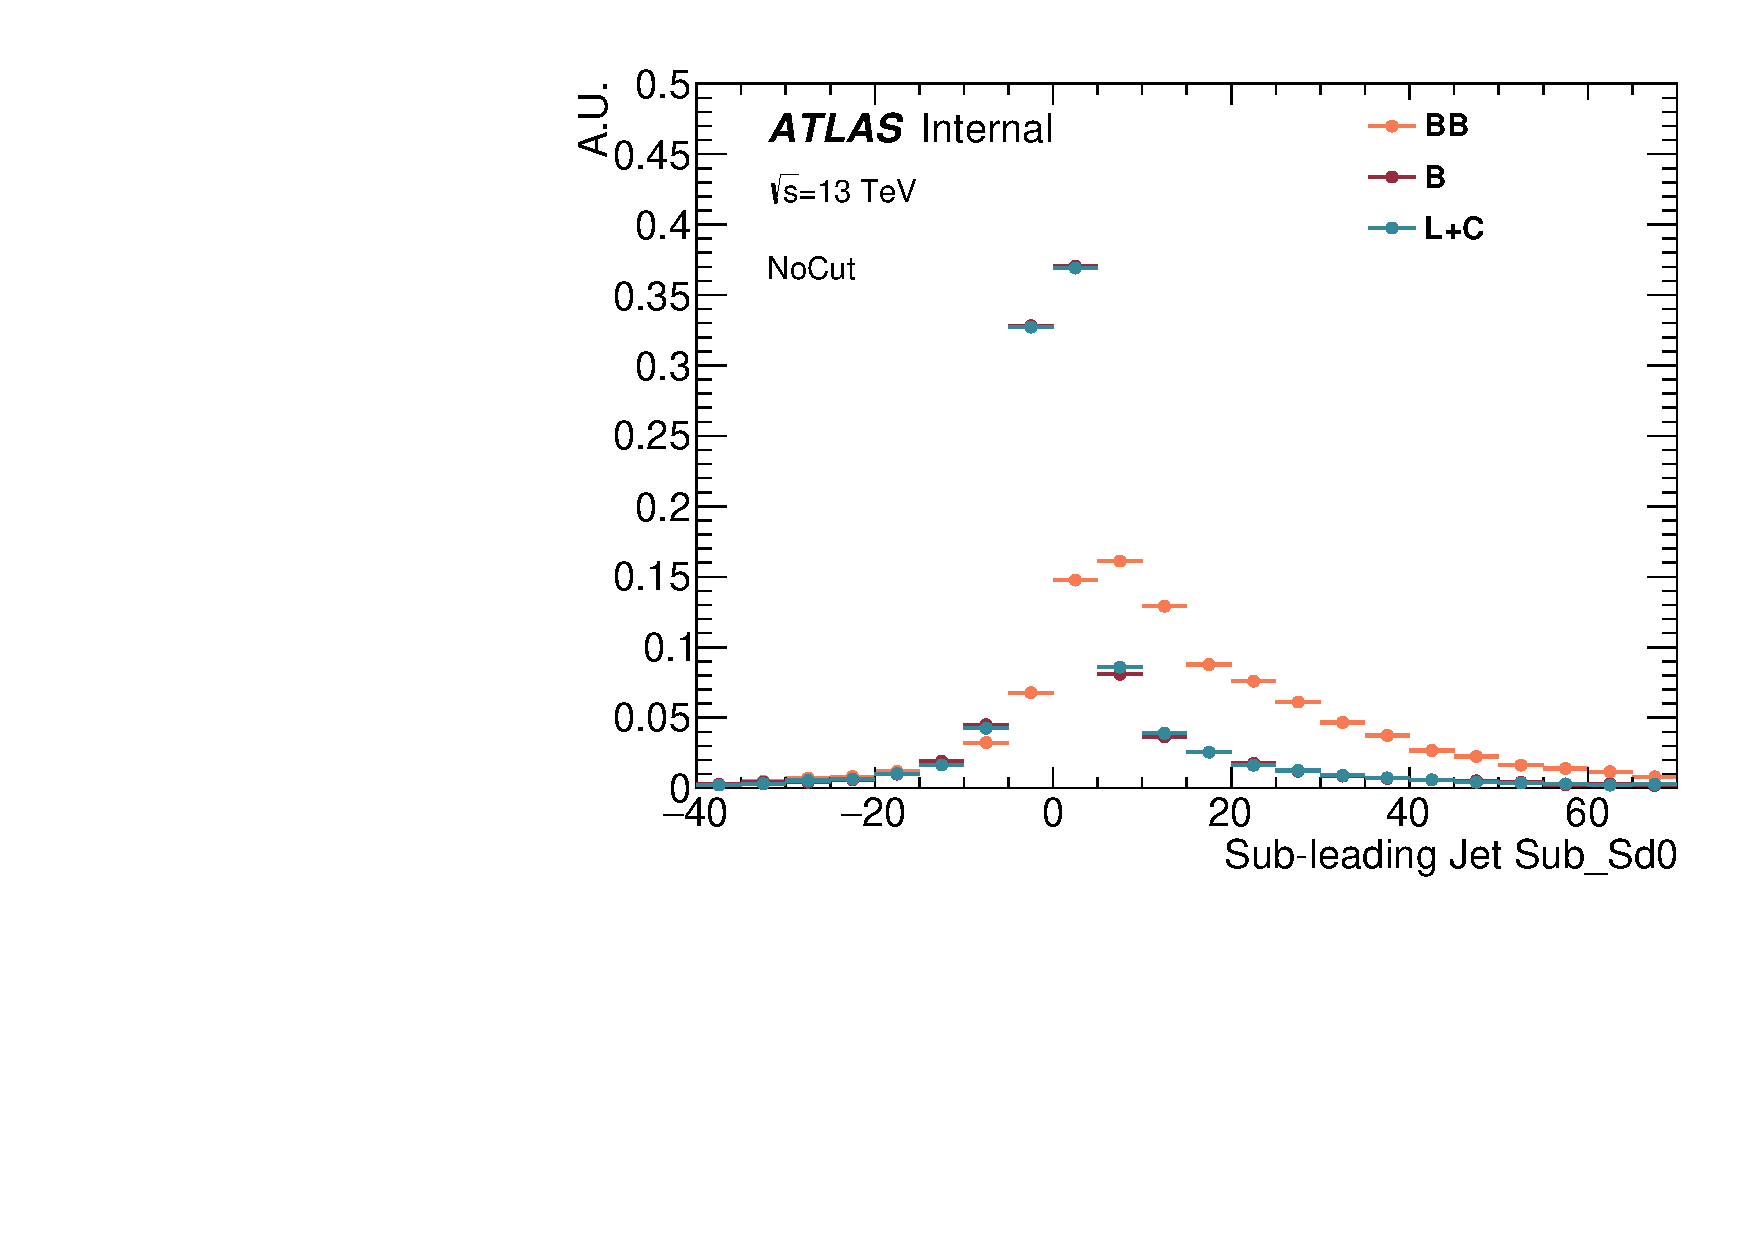
\includegraphics[width=0.48\textwidth]{figures/gbb/Sub_Sd0_Fits/Canv_FitTemplate_Inclusive_y.pdf}\\
\caption{The merged \subsdzero templates (inclusive) for leading (left) and sub-leading (right) track jets.}
  \label{fig:gbb-templates}
\end{figure}


\begin{figure}[htbp]
  \centering
 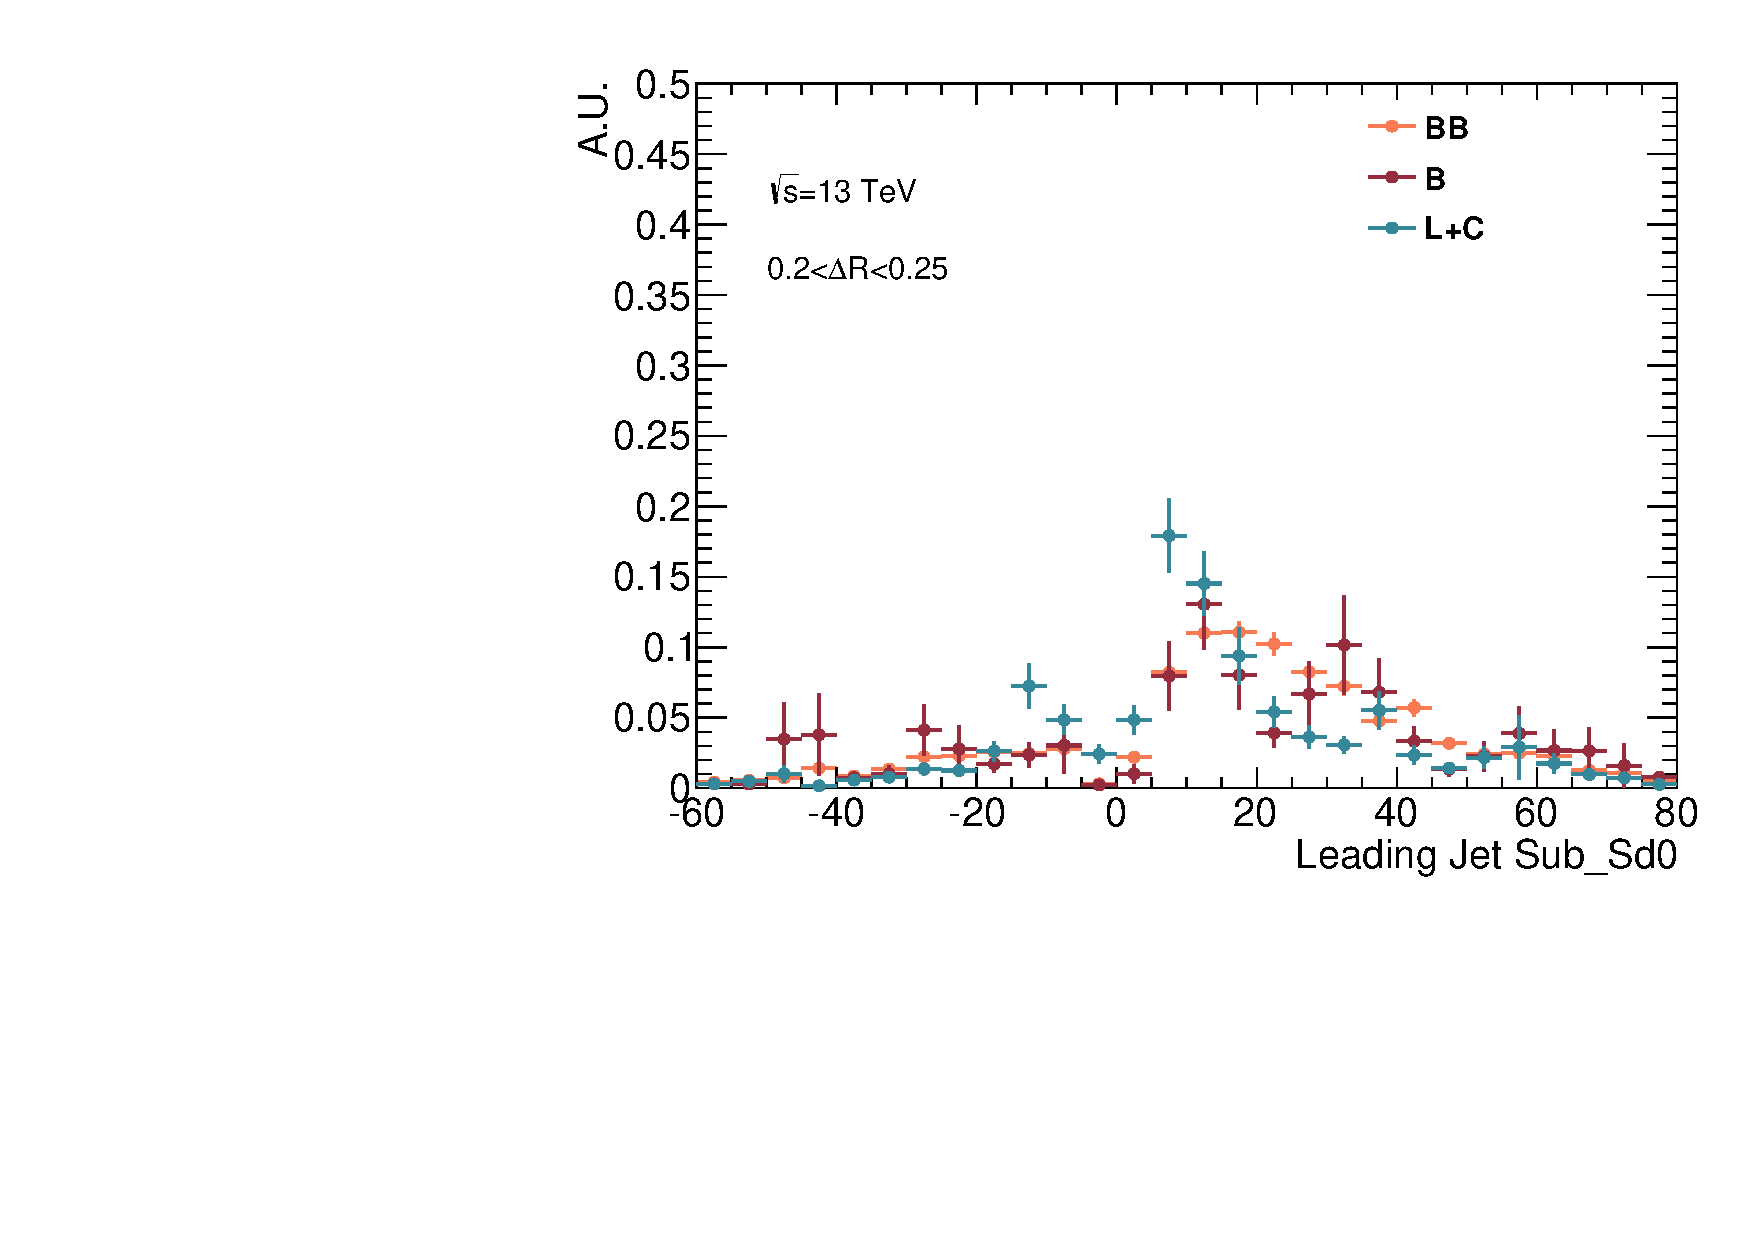
\includegraphics[width=0.48\textwidth]{figures/gbb/Canv_FitTemplate_medium.pdf}
 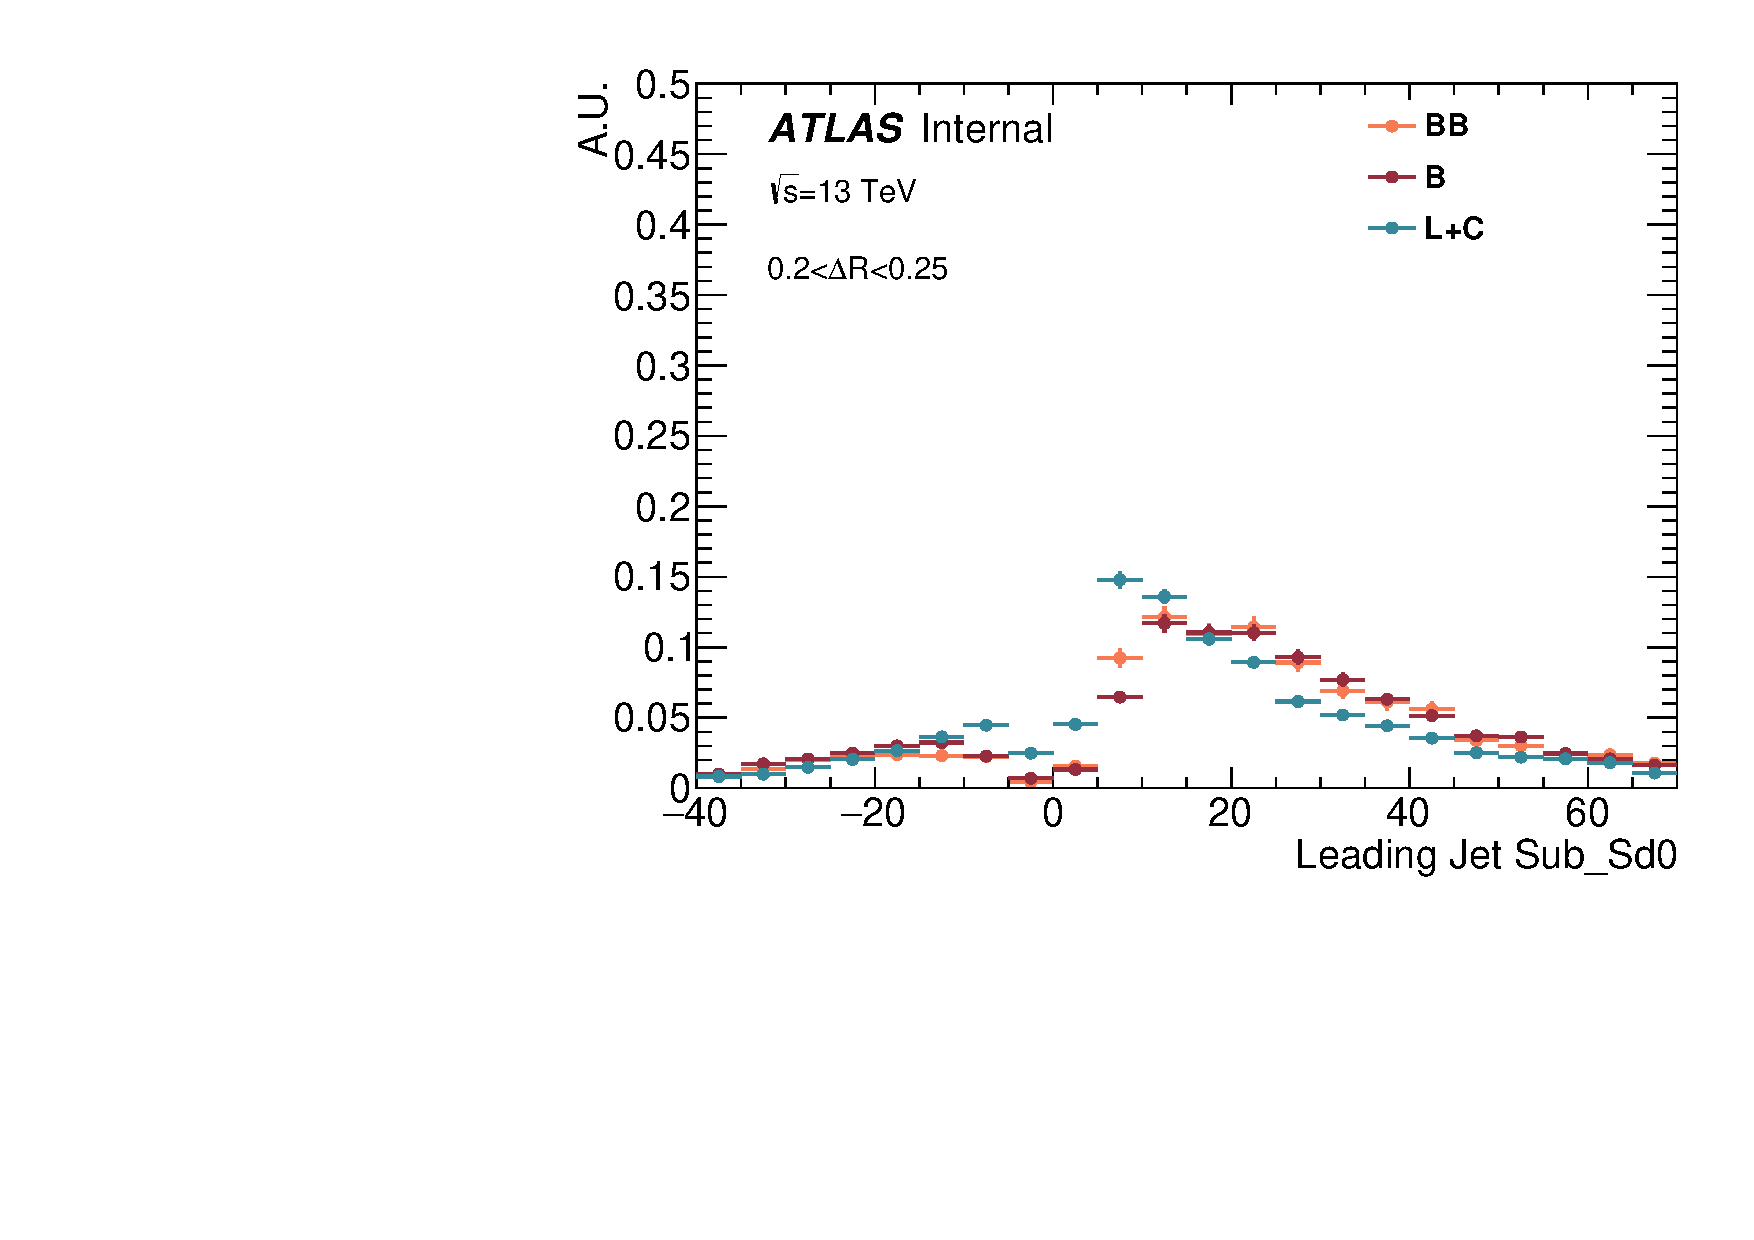
\includegraphics[width=0.48\textwidth]{figures/gbb/Sub_Sd0_Fits/Canv_FitTemplate_02-DeltaR-025_LpT_INF_SpT_INF_x.pdf}\\
\caption{The merged \subsdzero templates for leading track jets of events with $0.2<\Delta R<0.25$ for double $b$-tagging at 70\% eff WP (left) and single $b$-tagging (right). Post double $b$-tagging the statistics of background templates is too low.}
 \label{fig:gbb-template-leadtight-medium}
\end{figure}


%%%%%%%%%%%%%%%%%%%%%%%%%%%%%%%
\subsection{Systematic Uncertainty from Flavor Fraction Fits and Validation Checks}
\label{sec:gbb-sub_systematics}

Separate fits are performed for all the $\pm 1\sigma$ variations of detector systematics listed in Section~\ref{sec:gbb-systs:exp} and propagated through fits. In addition, a number of systematic uncertainties specific for the flavor fraction fits are taken into account for the background determination of the nominal fit:

\begin{enumerate}
  \item \textbf{Data and MC statistical uncertainties:} The fit statistical uncertainties are taken directly from the errors from the MINUIT fitting package and propagated to unfolding.
  \item \textbf{Fit range:} The nominal flavor fraction fit is performed in \subsdzero$\in[-40, 70]$. To avoid having the potential tail mis-modeling of \subsdzero affects the result, fits are separately performed excluding the tails on the left $[-40, -30]$ and right side $[60, 70]$ of the \subsdzero distributions. The $b\bar b$ fitted fraction differences between the left/right-excluded fits and the nominal fit are propagated to unfolding machinery as one source of uncertainty. 
  \item \textbf{Template merging scheme:} The merge of small components to form aggregated templates essentially fixes the relative fractions of these components. The systematic uncertainties caused by the merging scheme is estimated by varying the contribution of each merged component up and down by a factor of two. The template fits are performed for each of these variations. In total $8\times 2 =16$ such variations are propagated to unfolding.
  \item \textbf{Alternative discriminants:} The robustness of the choice using \subsdzero as our fitting templates is checked against another choice using the leading and third-leading $s_{d0}$ value of the track jets, which we define as \sdzero and \subsubsdzero respectively. Note that fitting with these two different variables serves only as a closure check for different background modeling. The difference of fitted flavor fractions are not propagated as a systematic uncertainty associated with unfolding.
  \item \textbf{Fitting with \pt parameterized templates:} The nominal flavor fraction fit with inclusive \subsdzero templates are checked against fitting templates parameterized with track jets \pt. For each bin of observable, the flavor fraction fit is performed in four bins of leading (J1) and sub-leading (J2) track jet \pt: $(p_T(J1), p_T(J2))$. The four bins are $(p_T(J1)<200$~$\GeV, p_T(J2)<80$~$\GeV)$, $(p_T(J1)>200$~$\GeV, p_T(J2)<80$~$\GeV)$, $(p_T(J1)<200$~$\GeV, p_T(J2)>80$~$\GeV)$ and $(p_T(J1)>200$~~$\GeV, p_T(J2)>80$~$\GeV)$. The cross check is performed to check closure. The difference of fitted flavor fractions are not propagated as a systematic uncertainty associated with unfolding.
  \item \textbf{Kinematic re-weighting:} After the event selection, there are mild disagreements between data and MC of jet kinematic properties. The impact of the disagreement on the final results is explored by re-weighting the MC, event-by-event, by the ratio of the two dimensional leading and sub-leading track jets \pt and $\eta$ distributions between MC and data post \btagging as shown in Fig.~\ref{fig:gbb-reweightmap}. The mis-modeling could arise from the overall di-jet cross section, $R=1.0$ ghost matching efficiency and $b$-tagging efficiency as a function of \pt in the particular event topology. The data and MC comparison for the \pt of the $R=1.0$ and track jets are shown after applying $b$-tagging with and without kinematics re-weighting in Fig.~\ref{fig:gbb-pT_largeR},\ref{fig:gbb-pT_leadtrkjets},\ref{fig:gbb-pT_subtrkjets}. We do not find the re-weighting affects the flavor fit in any significant way and hence do not apply the re-weighting for the nominal results and the difference of fitted flavor fractions are not propagated as a systematic uncertainty associated with unfolding.

%\ref{fig:gbb-eta_largeR} \ref{fig:gbb-eta_leadtrkjets},\ref{fig:gbb-eta_subtrkjets}. The effects of applying kinematics re-weighting is checked. A cross check is performed fitting data with templates derived from reweighted sample.

\end{enumerate}

\begin{figure}[htbp]
  \centering
 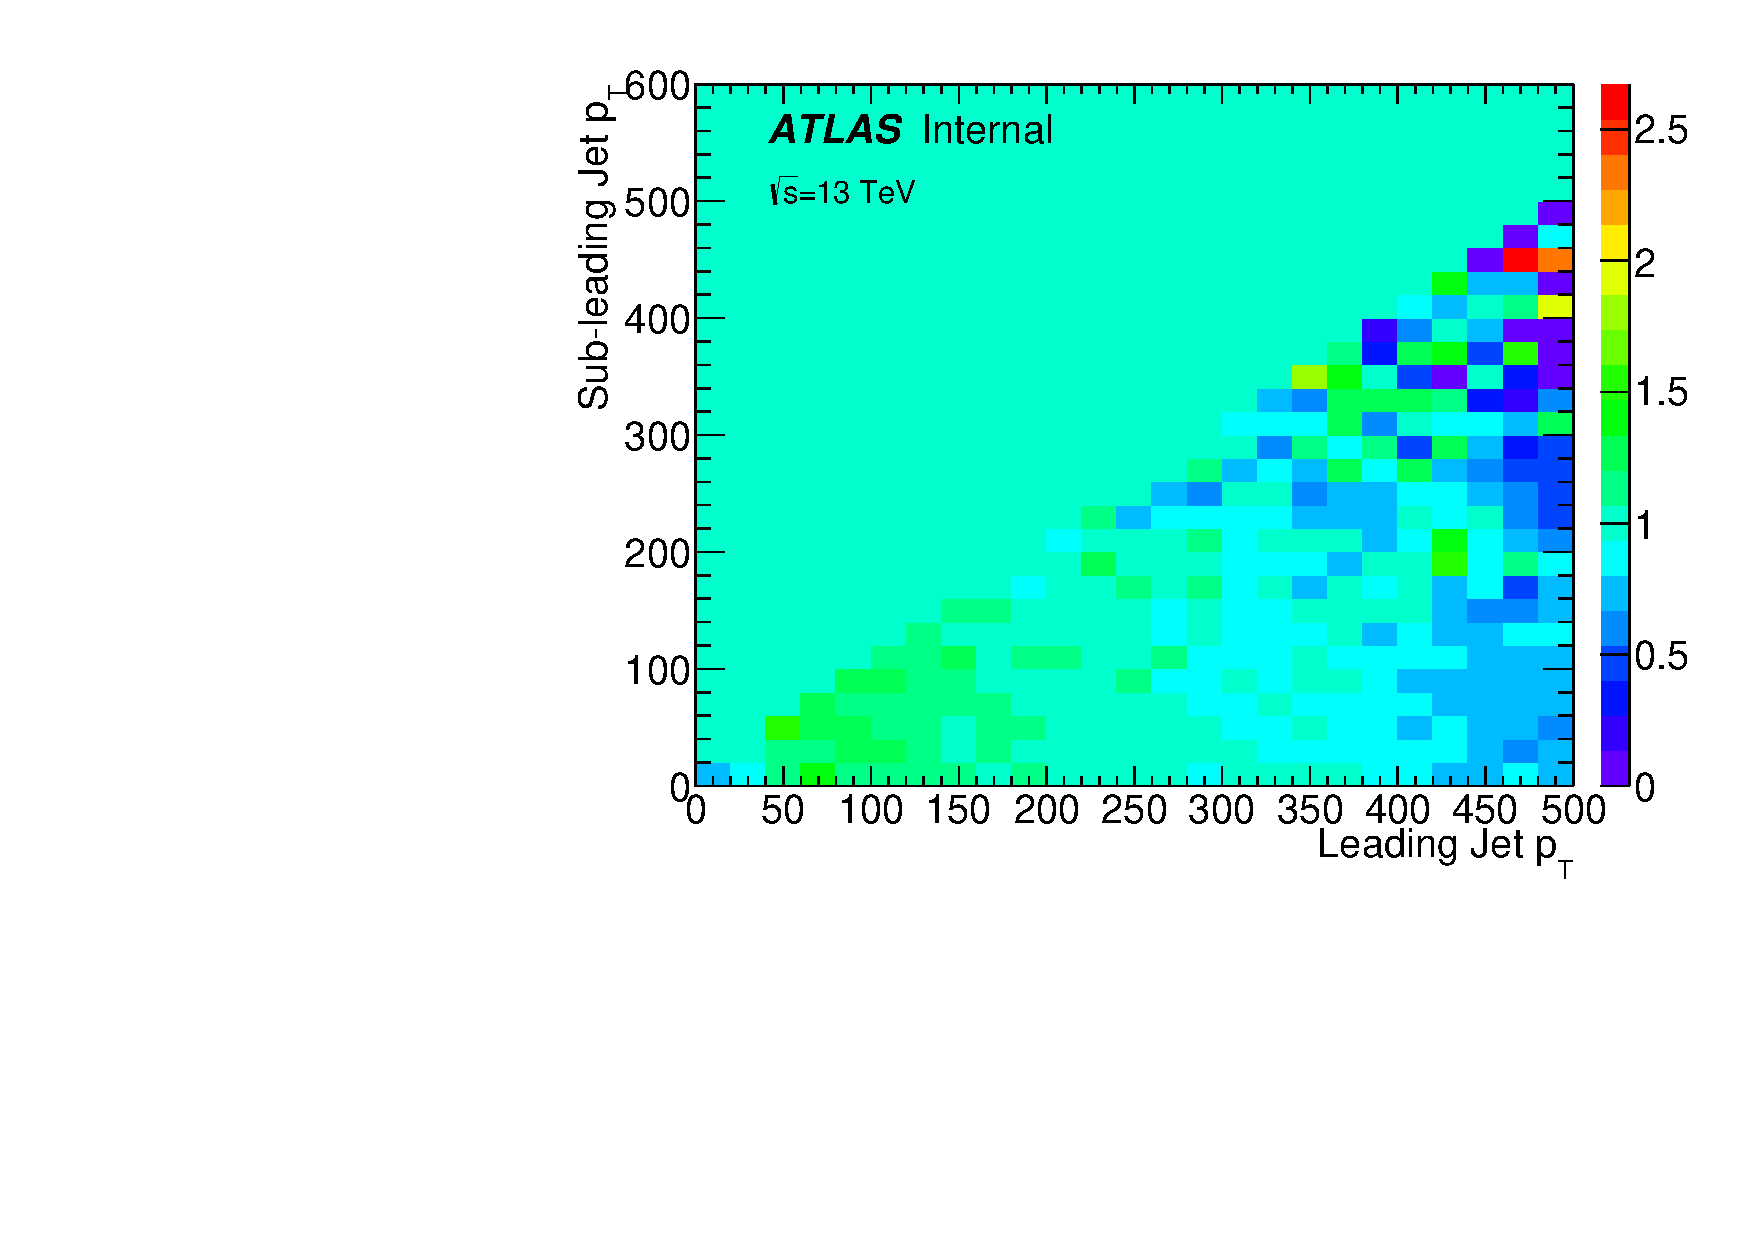
\includegraphics[width=0.6\textwidth]{figures/gbb/pTReweightMap.pdf}
\caption{The re-weighting factor applied to MC as a function of leading and sub-leading track jet \pt.}
  \label{fig:gbb-reweightmap}
\end{figure}


\begin{figure}[htbp]
  \centering
 %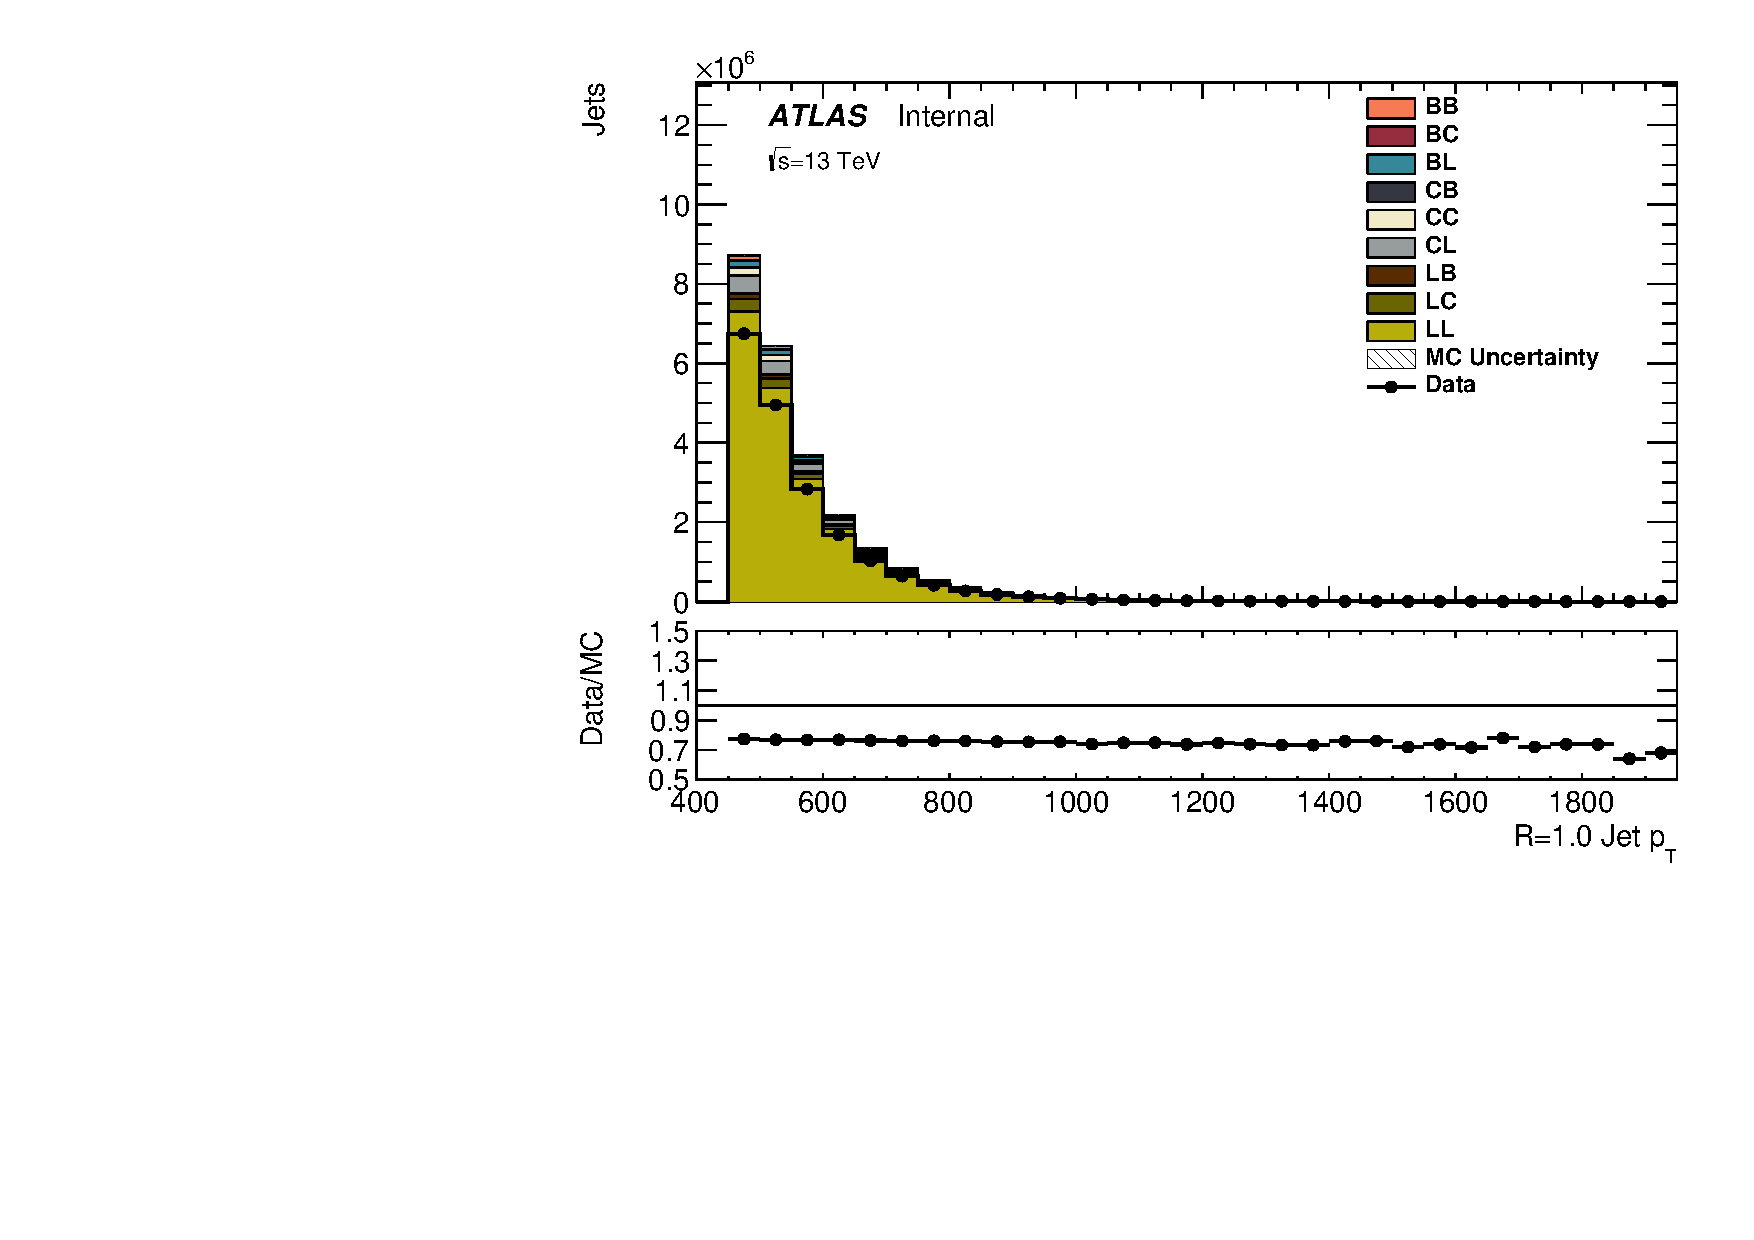
\includegraphics[width=0.38\textwidth]{figures/gbb/LargeRJet_pT_NoReweight.pdf}
 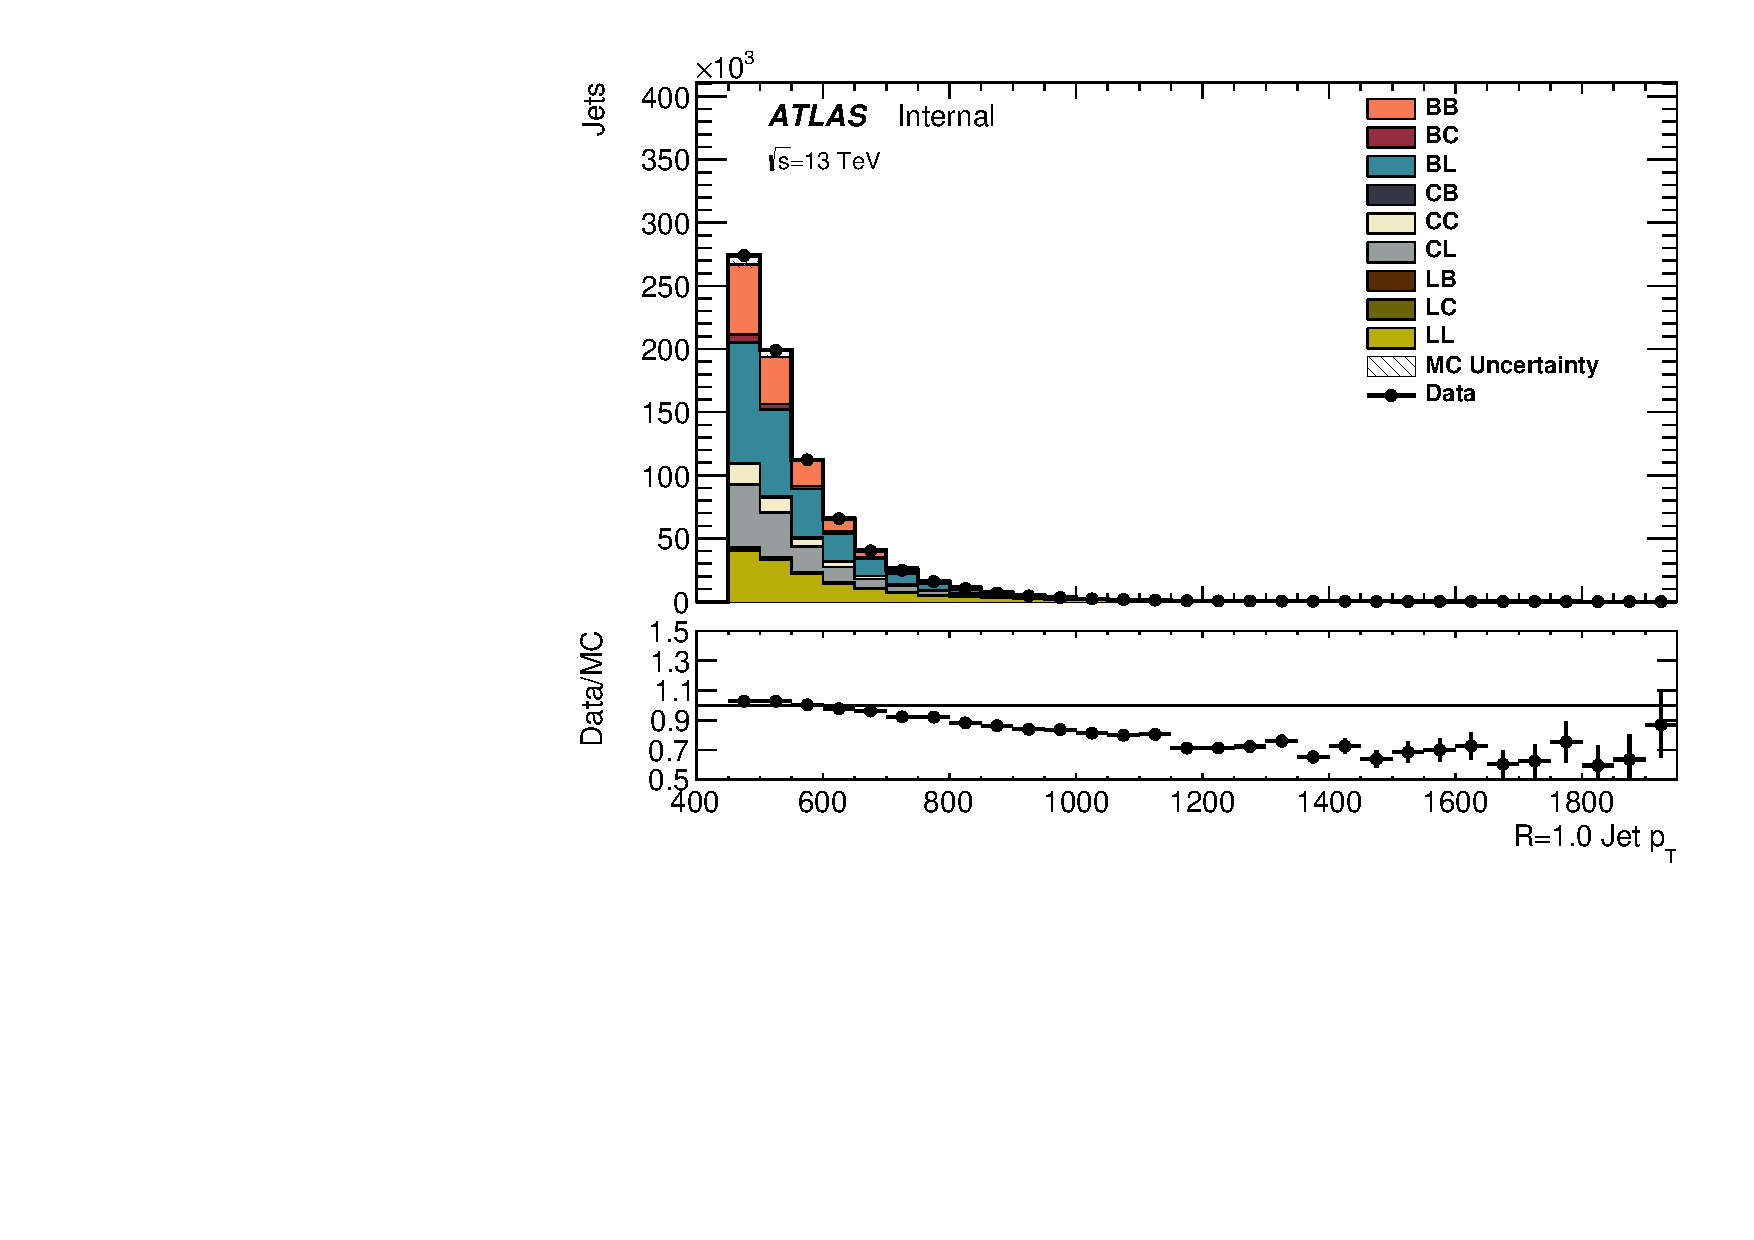
\includegraphics[width=0.38\textwidth]{figures/gbb/LargeRJet_pT_PreReweight.pdf}
 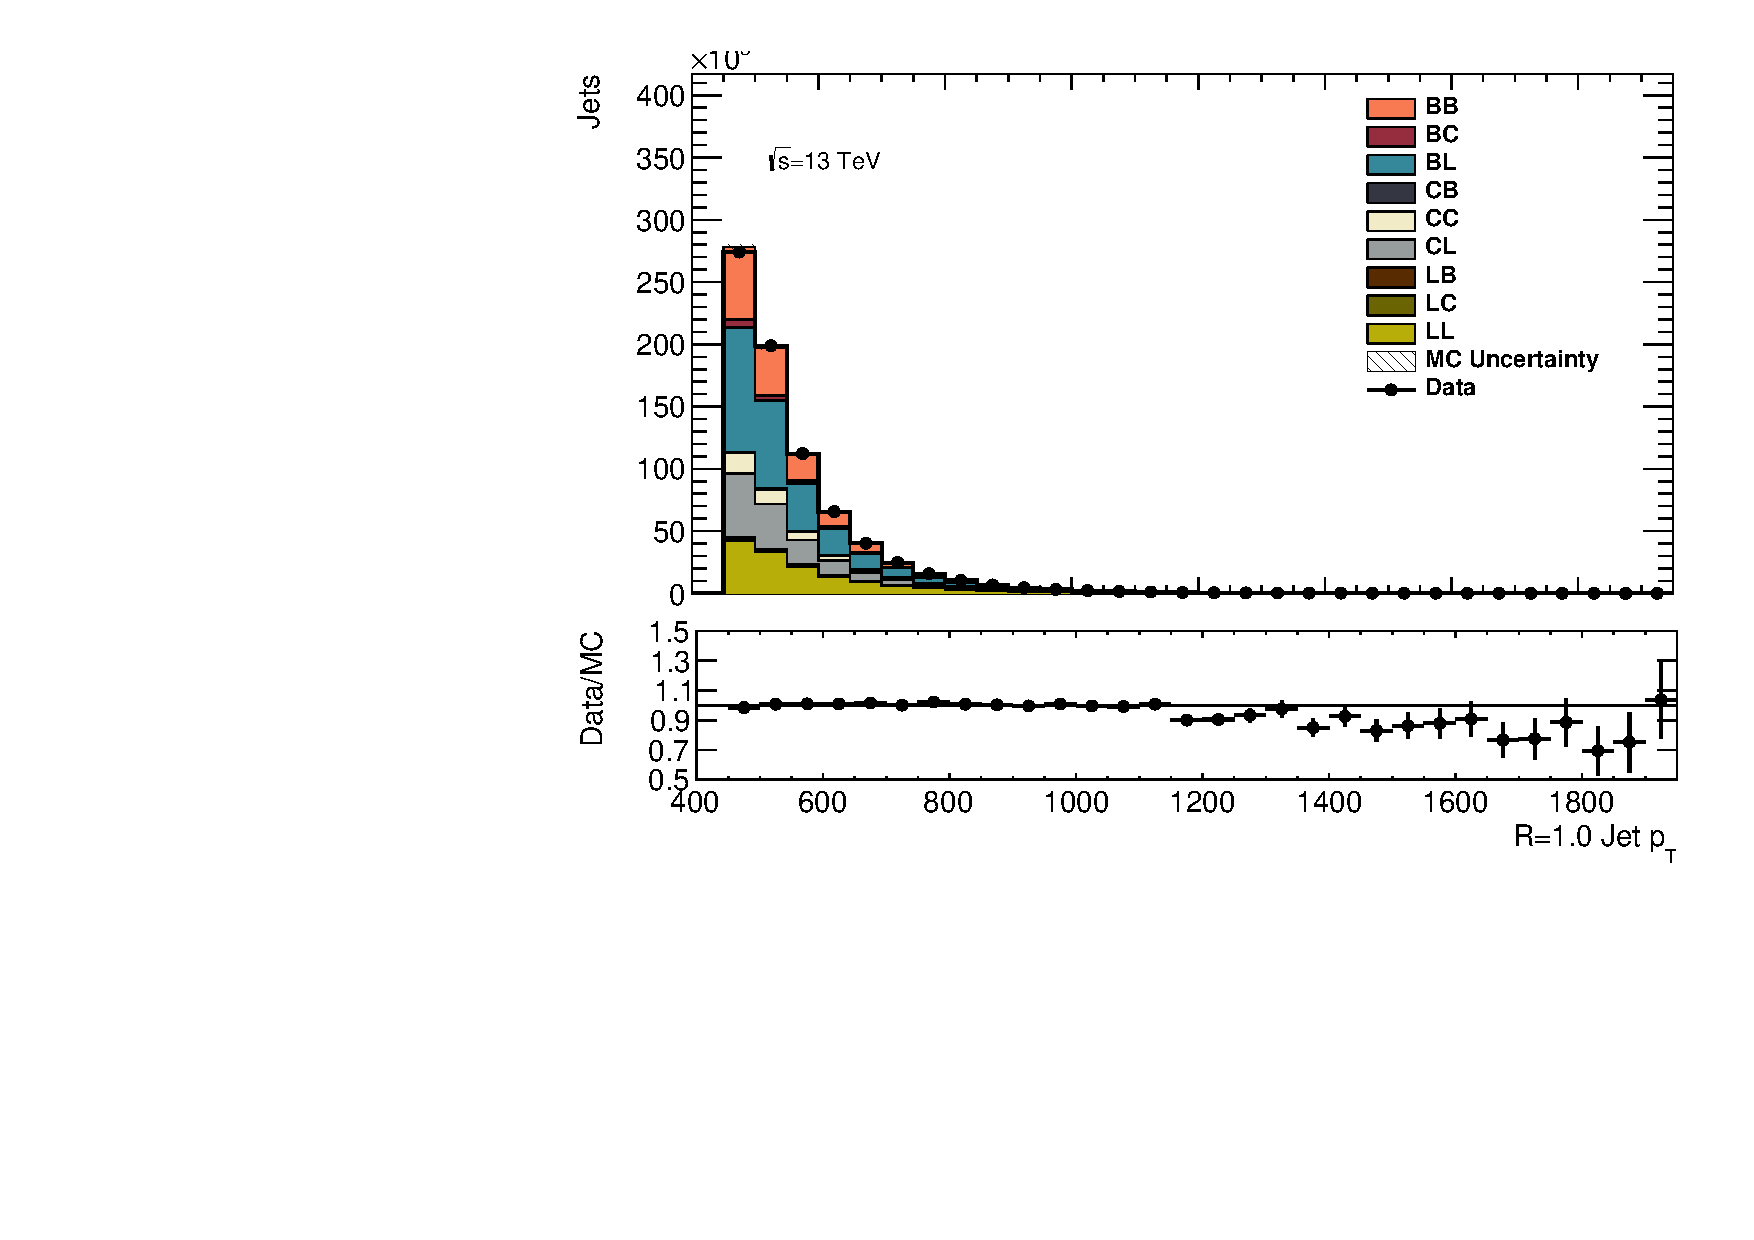
\includegraphics[width=0.38\textwidth]{figures/gbb/LargeRJet_pT_Reweight.pdf}
\caption{Data/MC comparison of $R=1.0$ jet post $b$-tagging without kinematic re-weighting (left) and post $b$-tagging with kinematic re-weighting (right).}% The label of the $R=1.0$ jet flavor content ``XY'' denotes the leading and sub-leading track jet flavor. For example, the flavors of the leading and sub-leading track jet of a ``BL'' $R=1.0$ jet are `B' and `Light' respectively.}
  \label{fig:gbb-pT_largeR}
\end{figure}


\begin{figure}[htbp]
  \centering
  %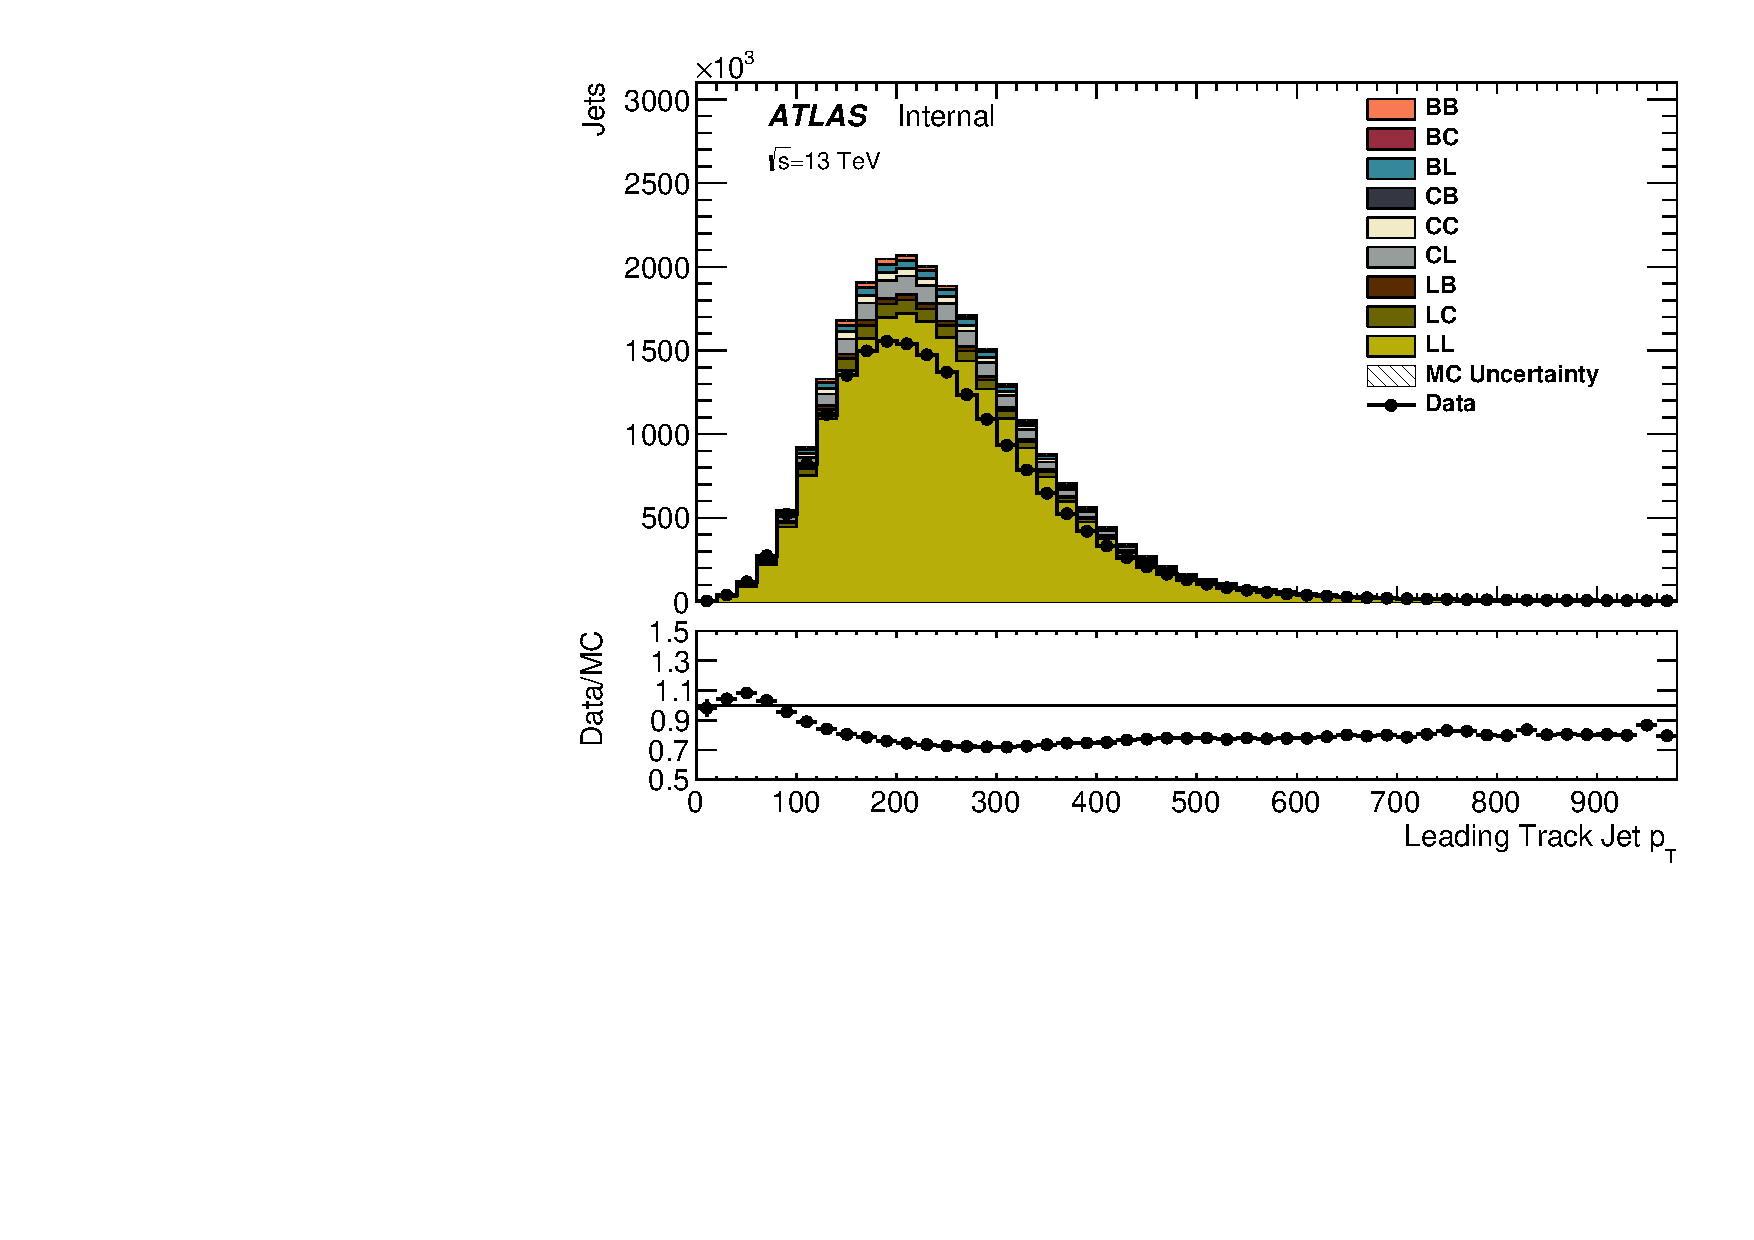
\includegraphics[width=0.38\textwidth]{figures/gbb/LeadTrkJet_pT_NoReweight.pdf}
 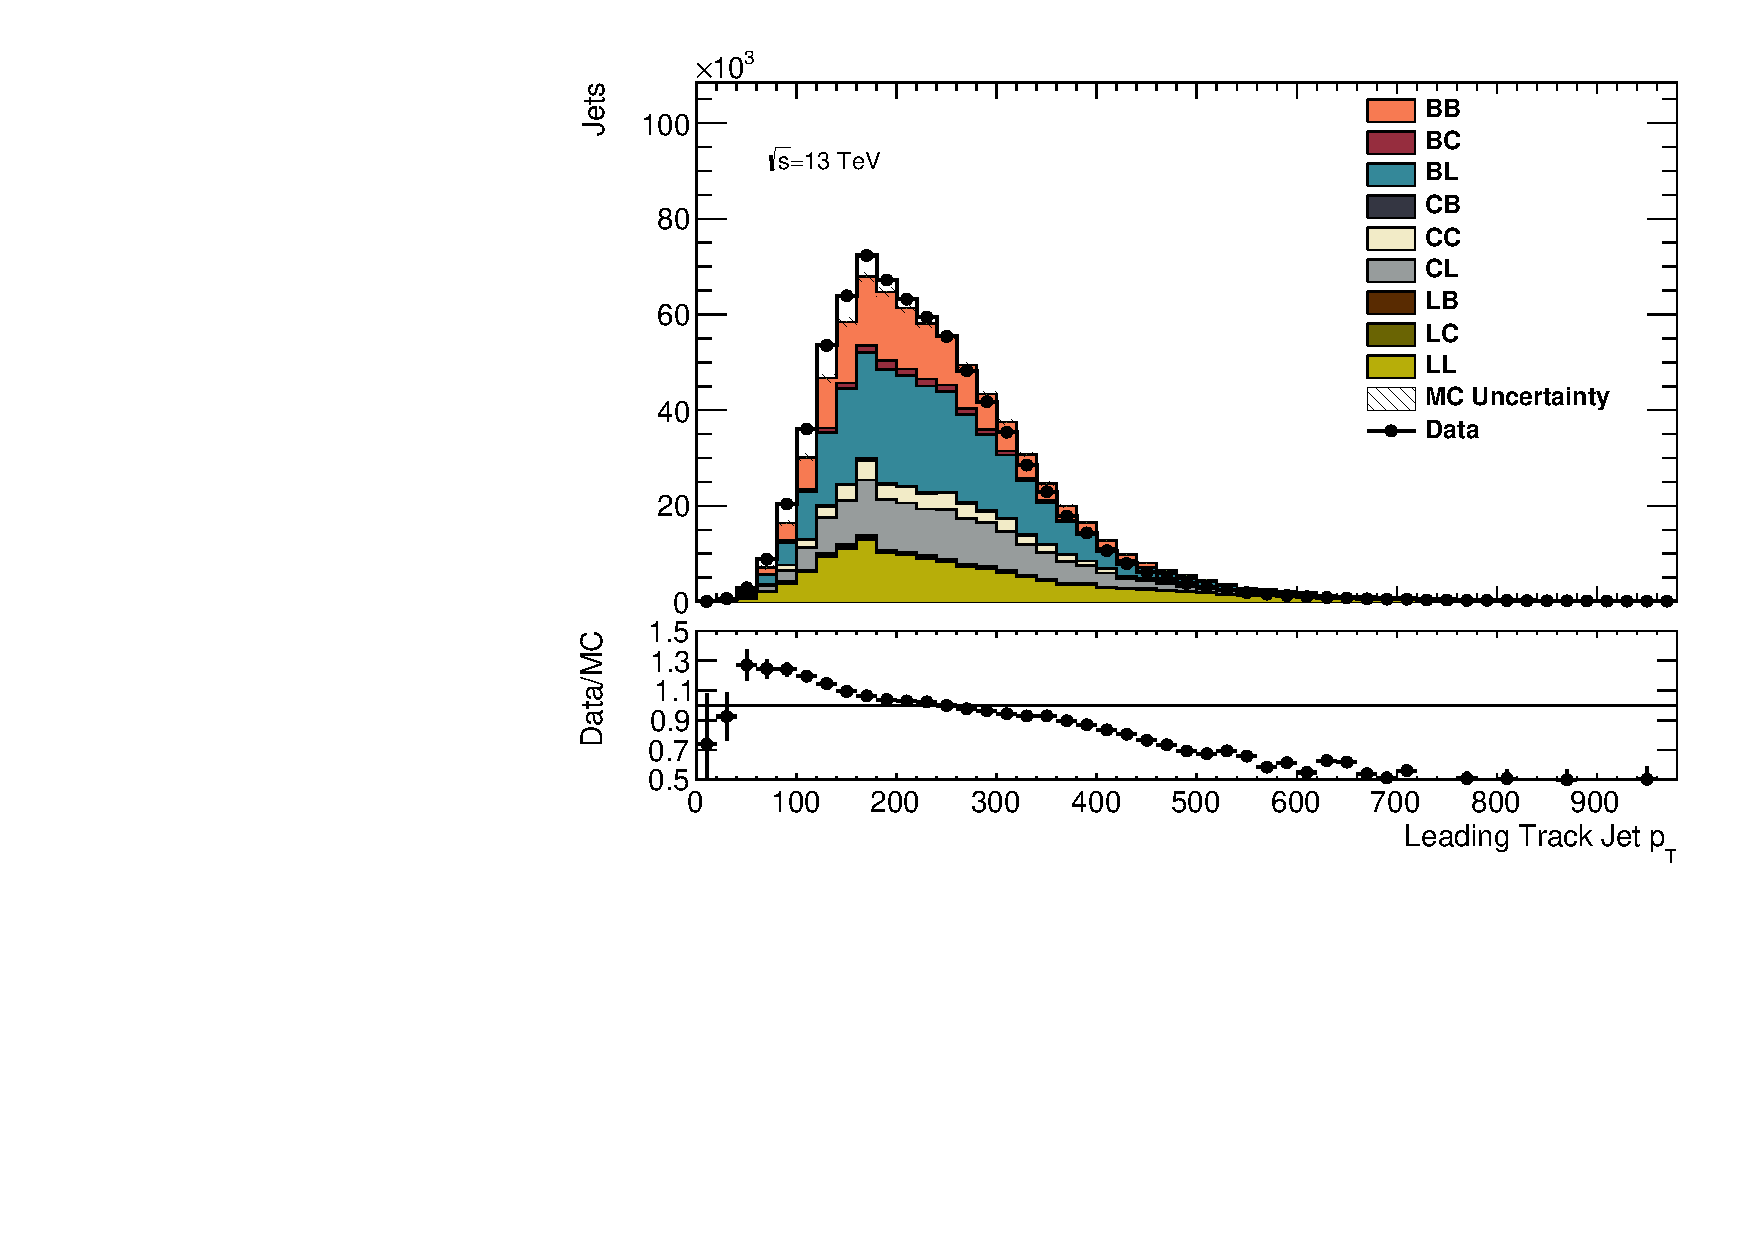
\includegraphics[width=0.38\textwidth]{figures/gbb/LeadTrkJet_pT_PreReweight.pdf}
 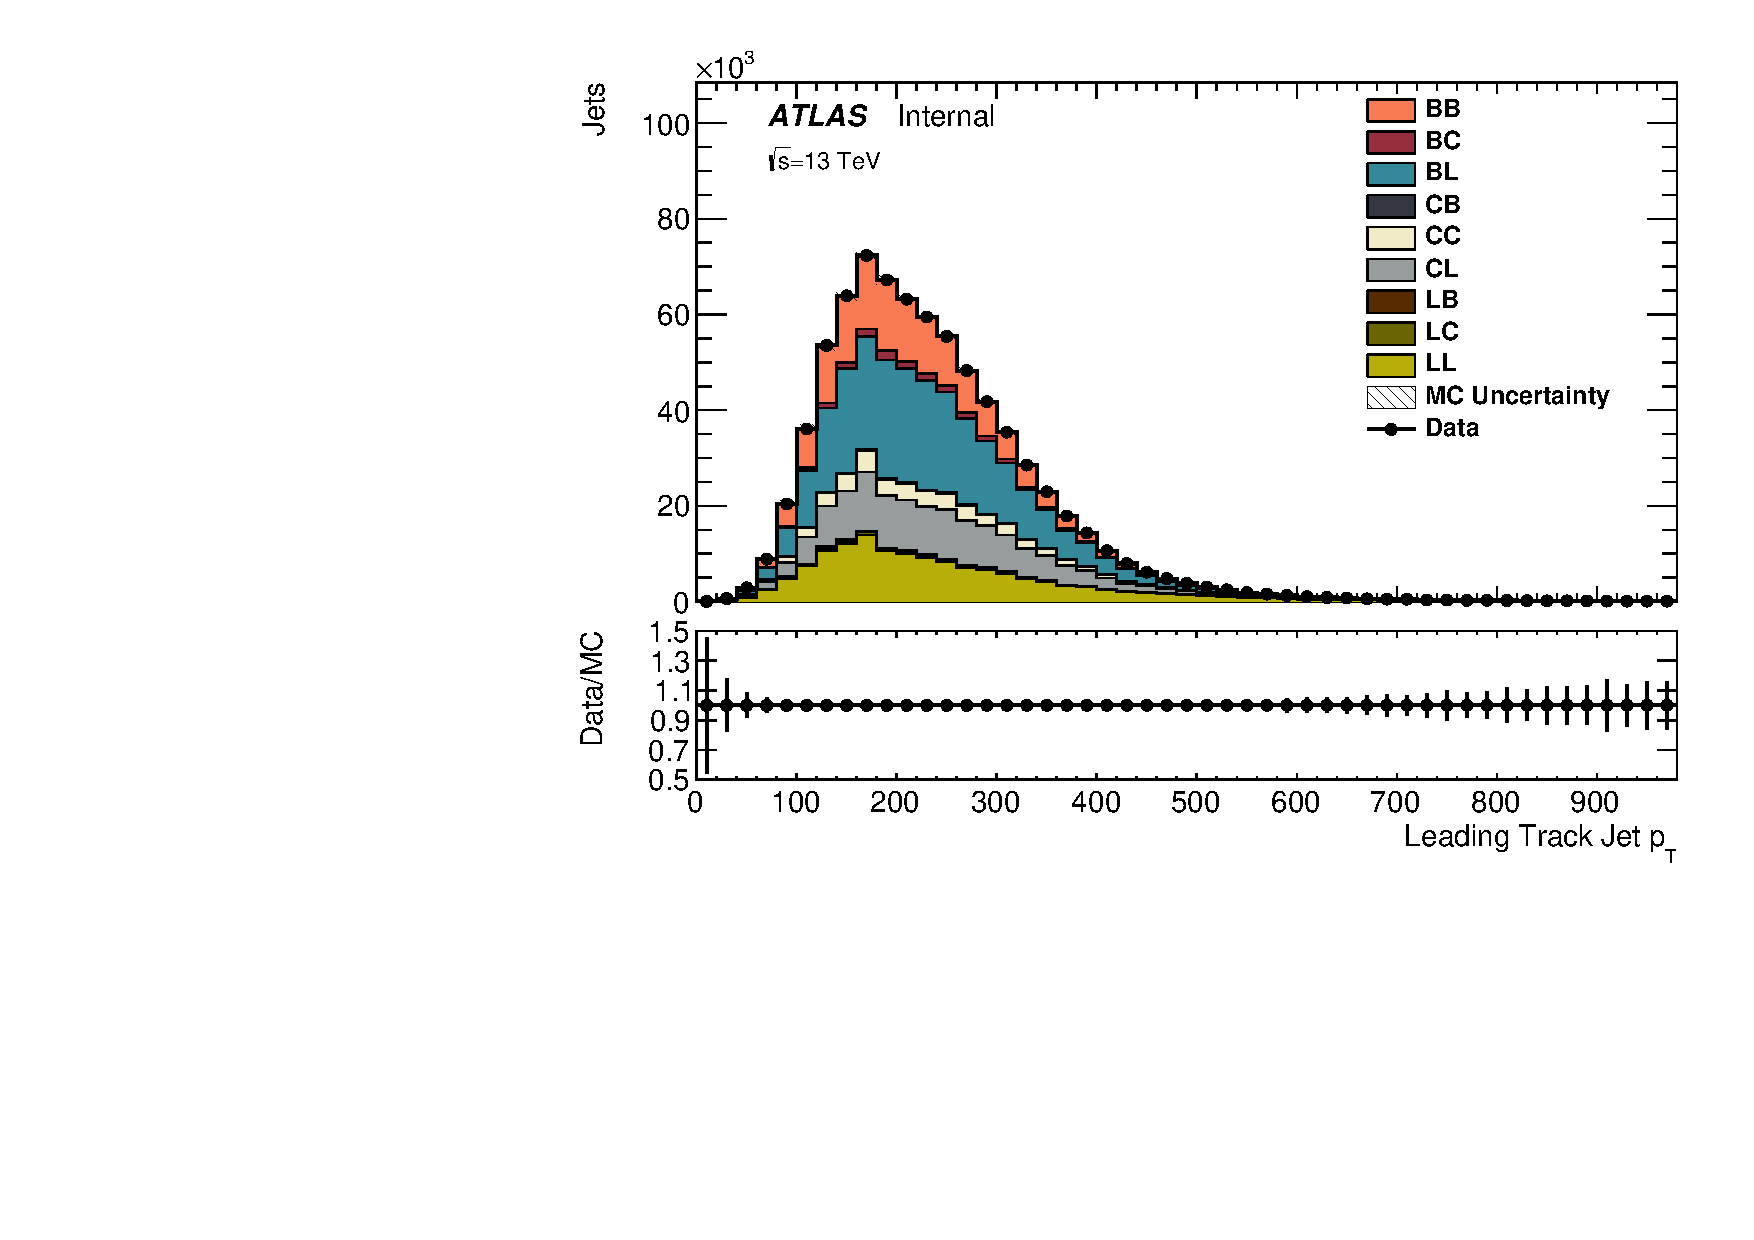
\includegraphics[width=0.38\textwidth]{figures/gbb/LeadTrkJet_pT_Reweight.pdf}
\caption{Data/MC comparison of leading track jets \pt post $b$-tagging without kinematic re-weighting (left) and post $b$-tagging with kinematic re-weighting (right).} % The label of the $R=1.0$ jet flavor content ``XY'' denotes the leading and sub-leading track jet flavor. For example, the flavors of the leading and sub-leading track jet of a ``BL'' $R=1.0$ jet are `B' and `Light' respectively.}
  \label{fig:gbb-pT_leadtrkjets}
\end{figure}


\begin{figure}[htbp]
  \centering
%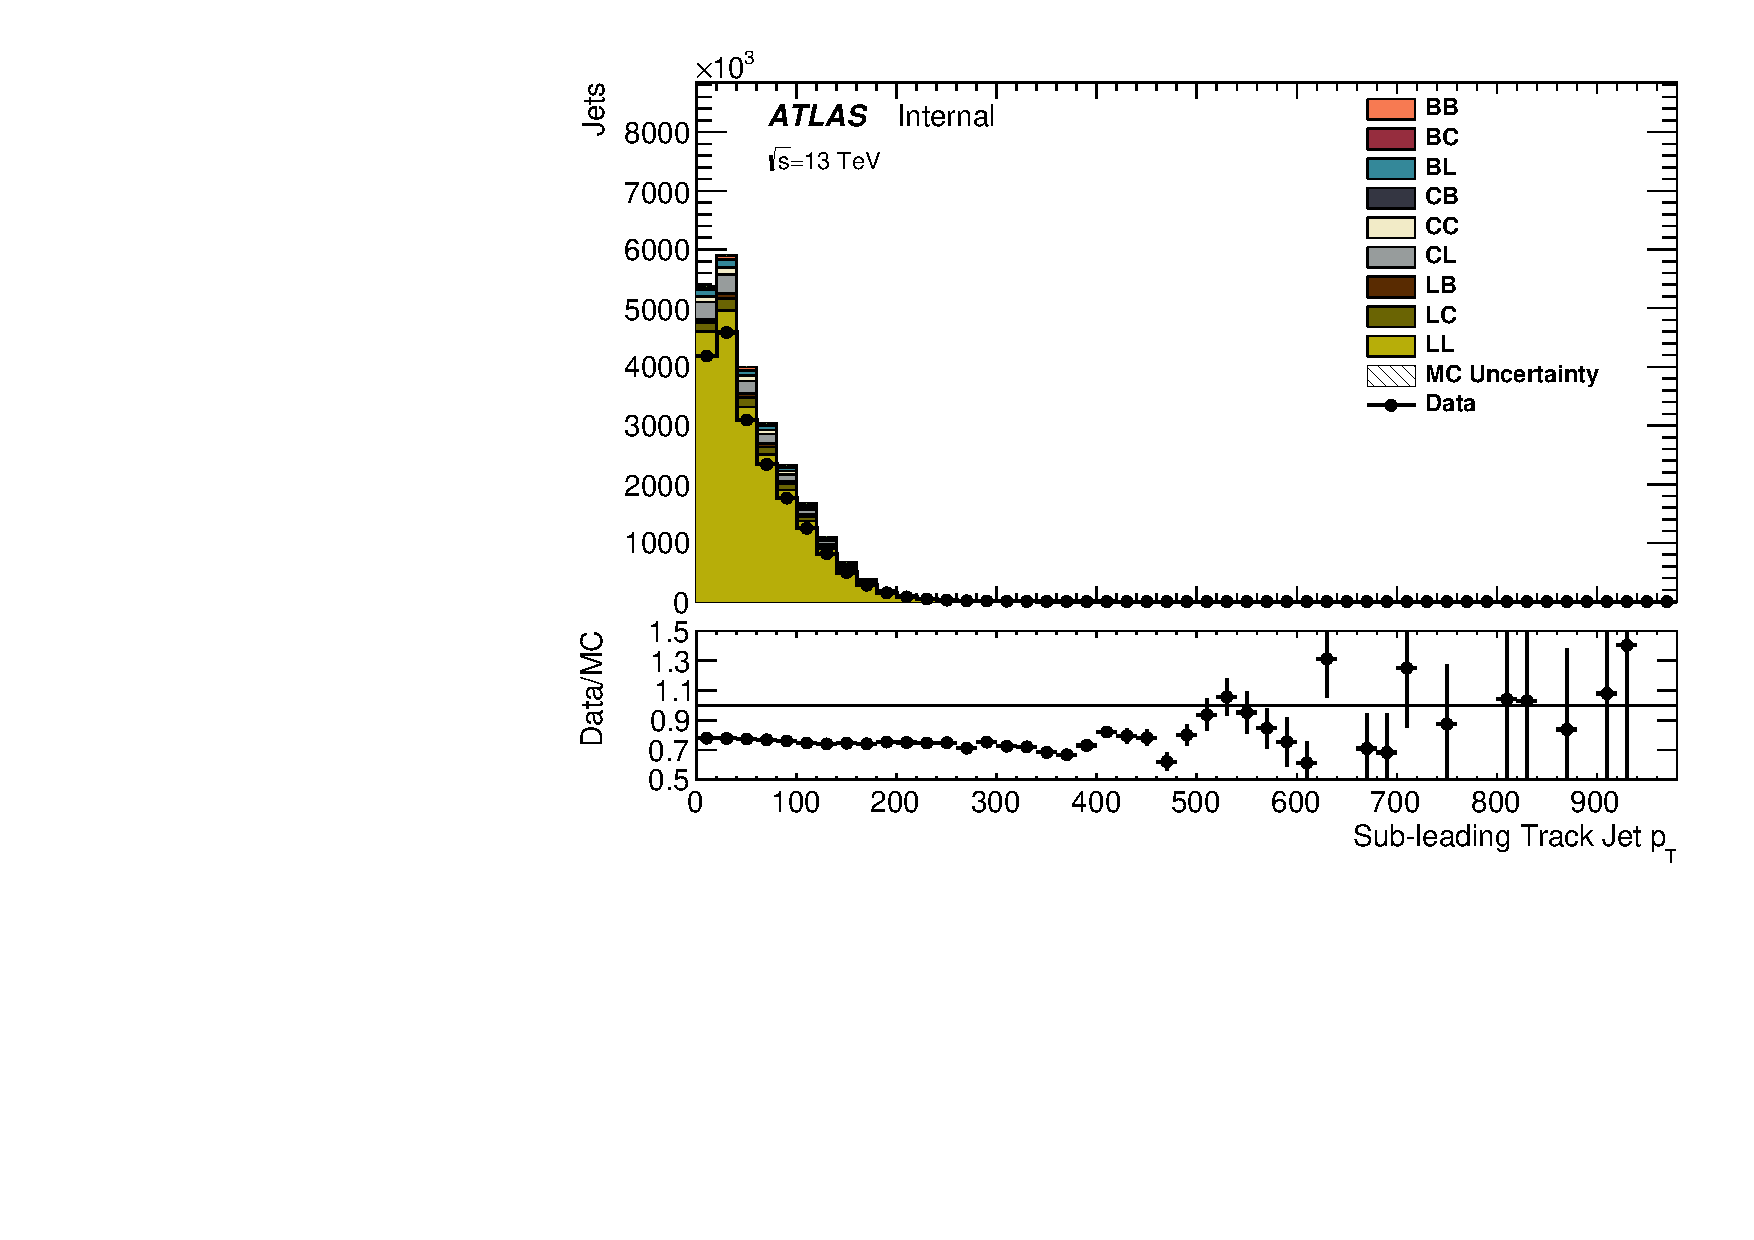
\includegraphics[width=0.38\textwidth]{figures/gbb/SubLeadTrkJet_pT_NoReweight.pdf}
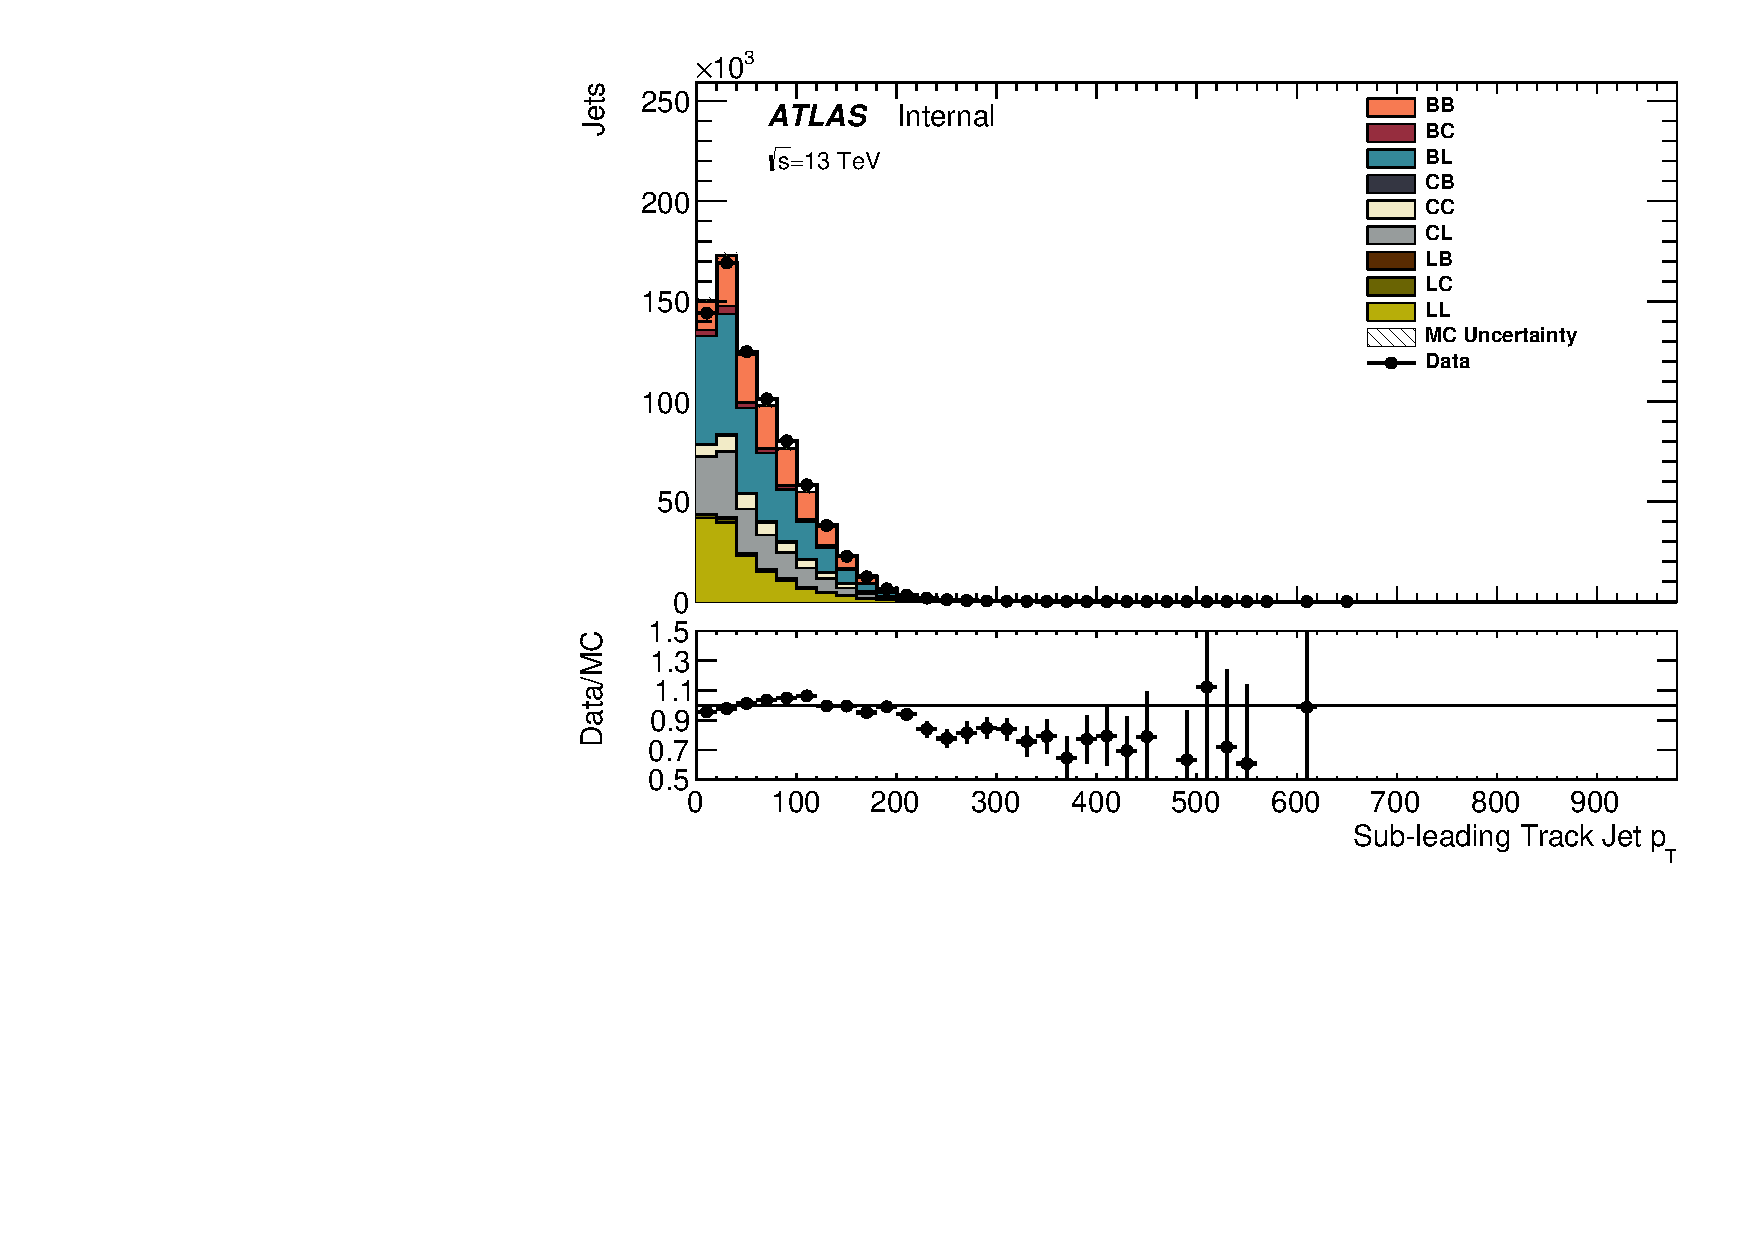
\includegraphics[width=0.38\textwidth]{figures/gbb/SubLeadTrkJet_pT_PreReweight.pdf}
 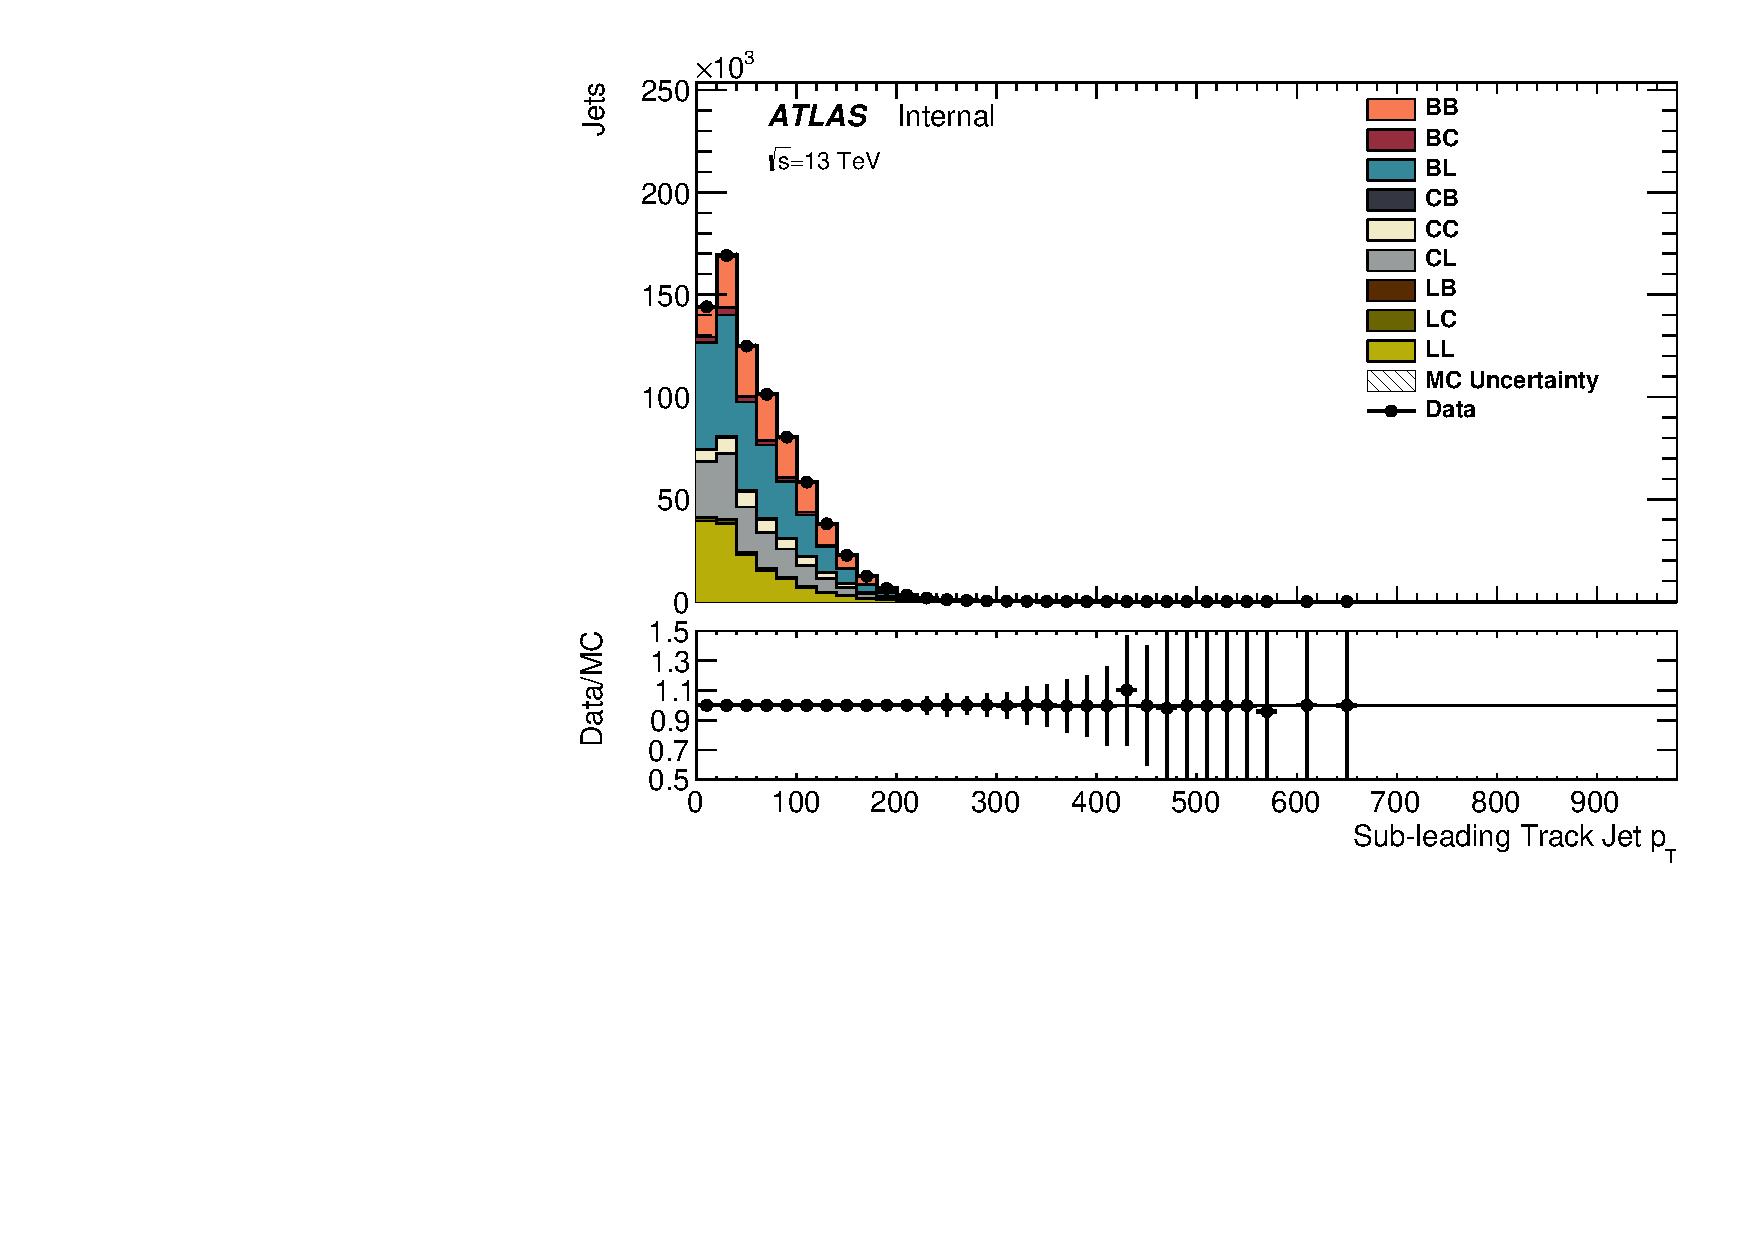
\includegraphics[width=0.38\textwidth]{figures/gbb/SubLeadTrkJet_pT_Reweight.pdf}
\caption{Data/MC comparison of sub-leading track jets \pt post $b$-tagging without kinematic re-weighting (left) and post $b$-tagging with kinematic re-weighting (right).}% The label of the $R=1.0$ jet flavor content ``XY'' denotes the leading and sub-leading track jet flavor. For example, the flavors of the leading and sub-leading track jet of a ``BL'' $R=1.0$ jet are `B' and `Light' respectively.}
  \label{fig:gbb-pT_subtrkjets}
\end{figure}
